\documentclass[../notes.tex]{subfiles}

\pagestyle{main}
\renewcommand{\chaptermark}[1]{\markboth{\chaptername\ \thechapter\ (#1)}{}}
\setcounter{chapter}{2}

\begin{document}




\chapter{Condensations}
\section{Problems 1, 4, and 8}
\begin{itemize}
    \item \marginnote{9/16:}David works with Rick Danheiser.
    \item We now begin discussing Problem 1.
    \begin{figure}[h!]
        \centering
        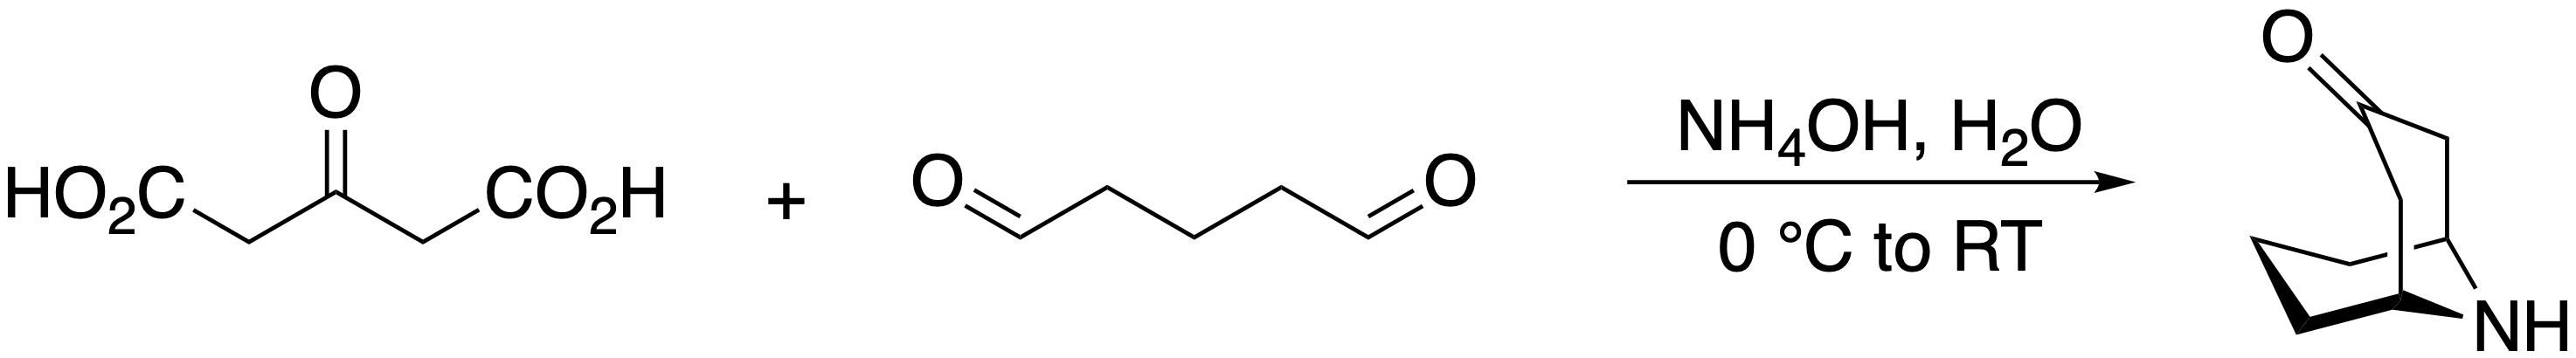
\includegraphics[width=0.6\linewidth]{WPSet1Q1.png}
        \caption{Wendlandt PSet 1, Q1.}
        \label{fig:WPSet1Q1}
    \end{figure}
    \item The reagents: \ce{NH4OH} in water is approximately $\pH=11$.
    \item Keto-enol tautomerization and amine condensation gets the carbons bonded in the right way.
    \begin{itemize}
        \item Dialdehyde forms an imine.
        \item The enol is not unreasonable because hydrogen bonding stabilizes a 6-membered ring.
        \item Then the enol can be a H-bond acceptor from the other carboxylate.
    \end{itemize}
    \item Watch out for reversible steps!!
    \item Loss of \ce{CO2} helps drive some of the steps.
    \item There are multiple right answers; David's sequence of events works, but others could be valid, too.
    \item Aldehyde is more electrophilic than the monoprotonated imine, so if we're gonna react with an imine, we need to change both aldehydes into imines first. Alternatively, we need to diprotonate the imine.
    \item It's not clear whether decarboxylation happens earlier or later in the mechanism.
    \item Altogether, the full solution to PSet 1, Q1 is on the next page.
    \begin{figure}[H]
        \centering
        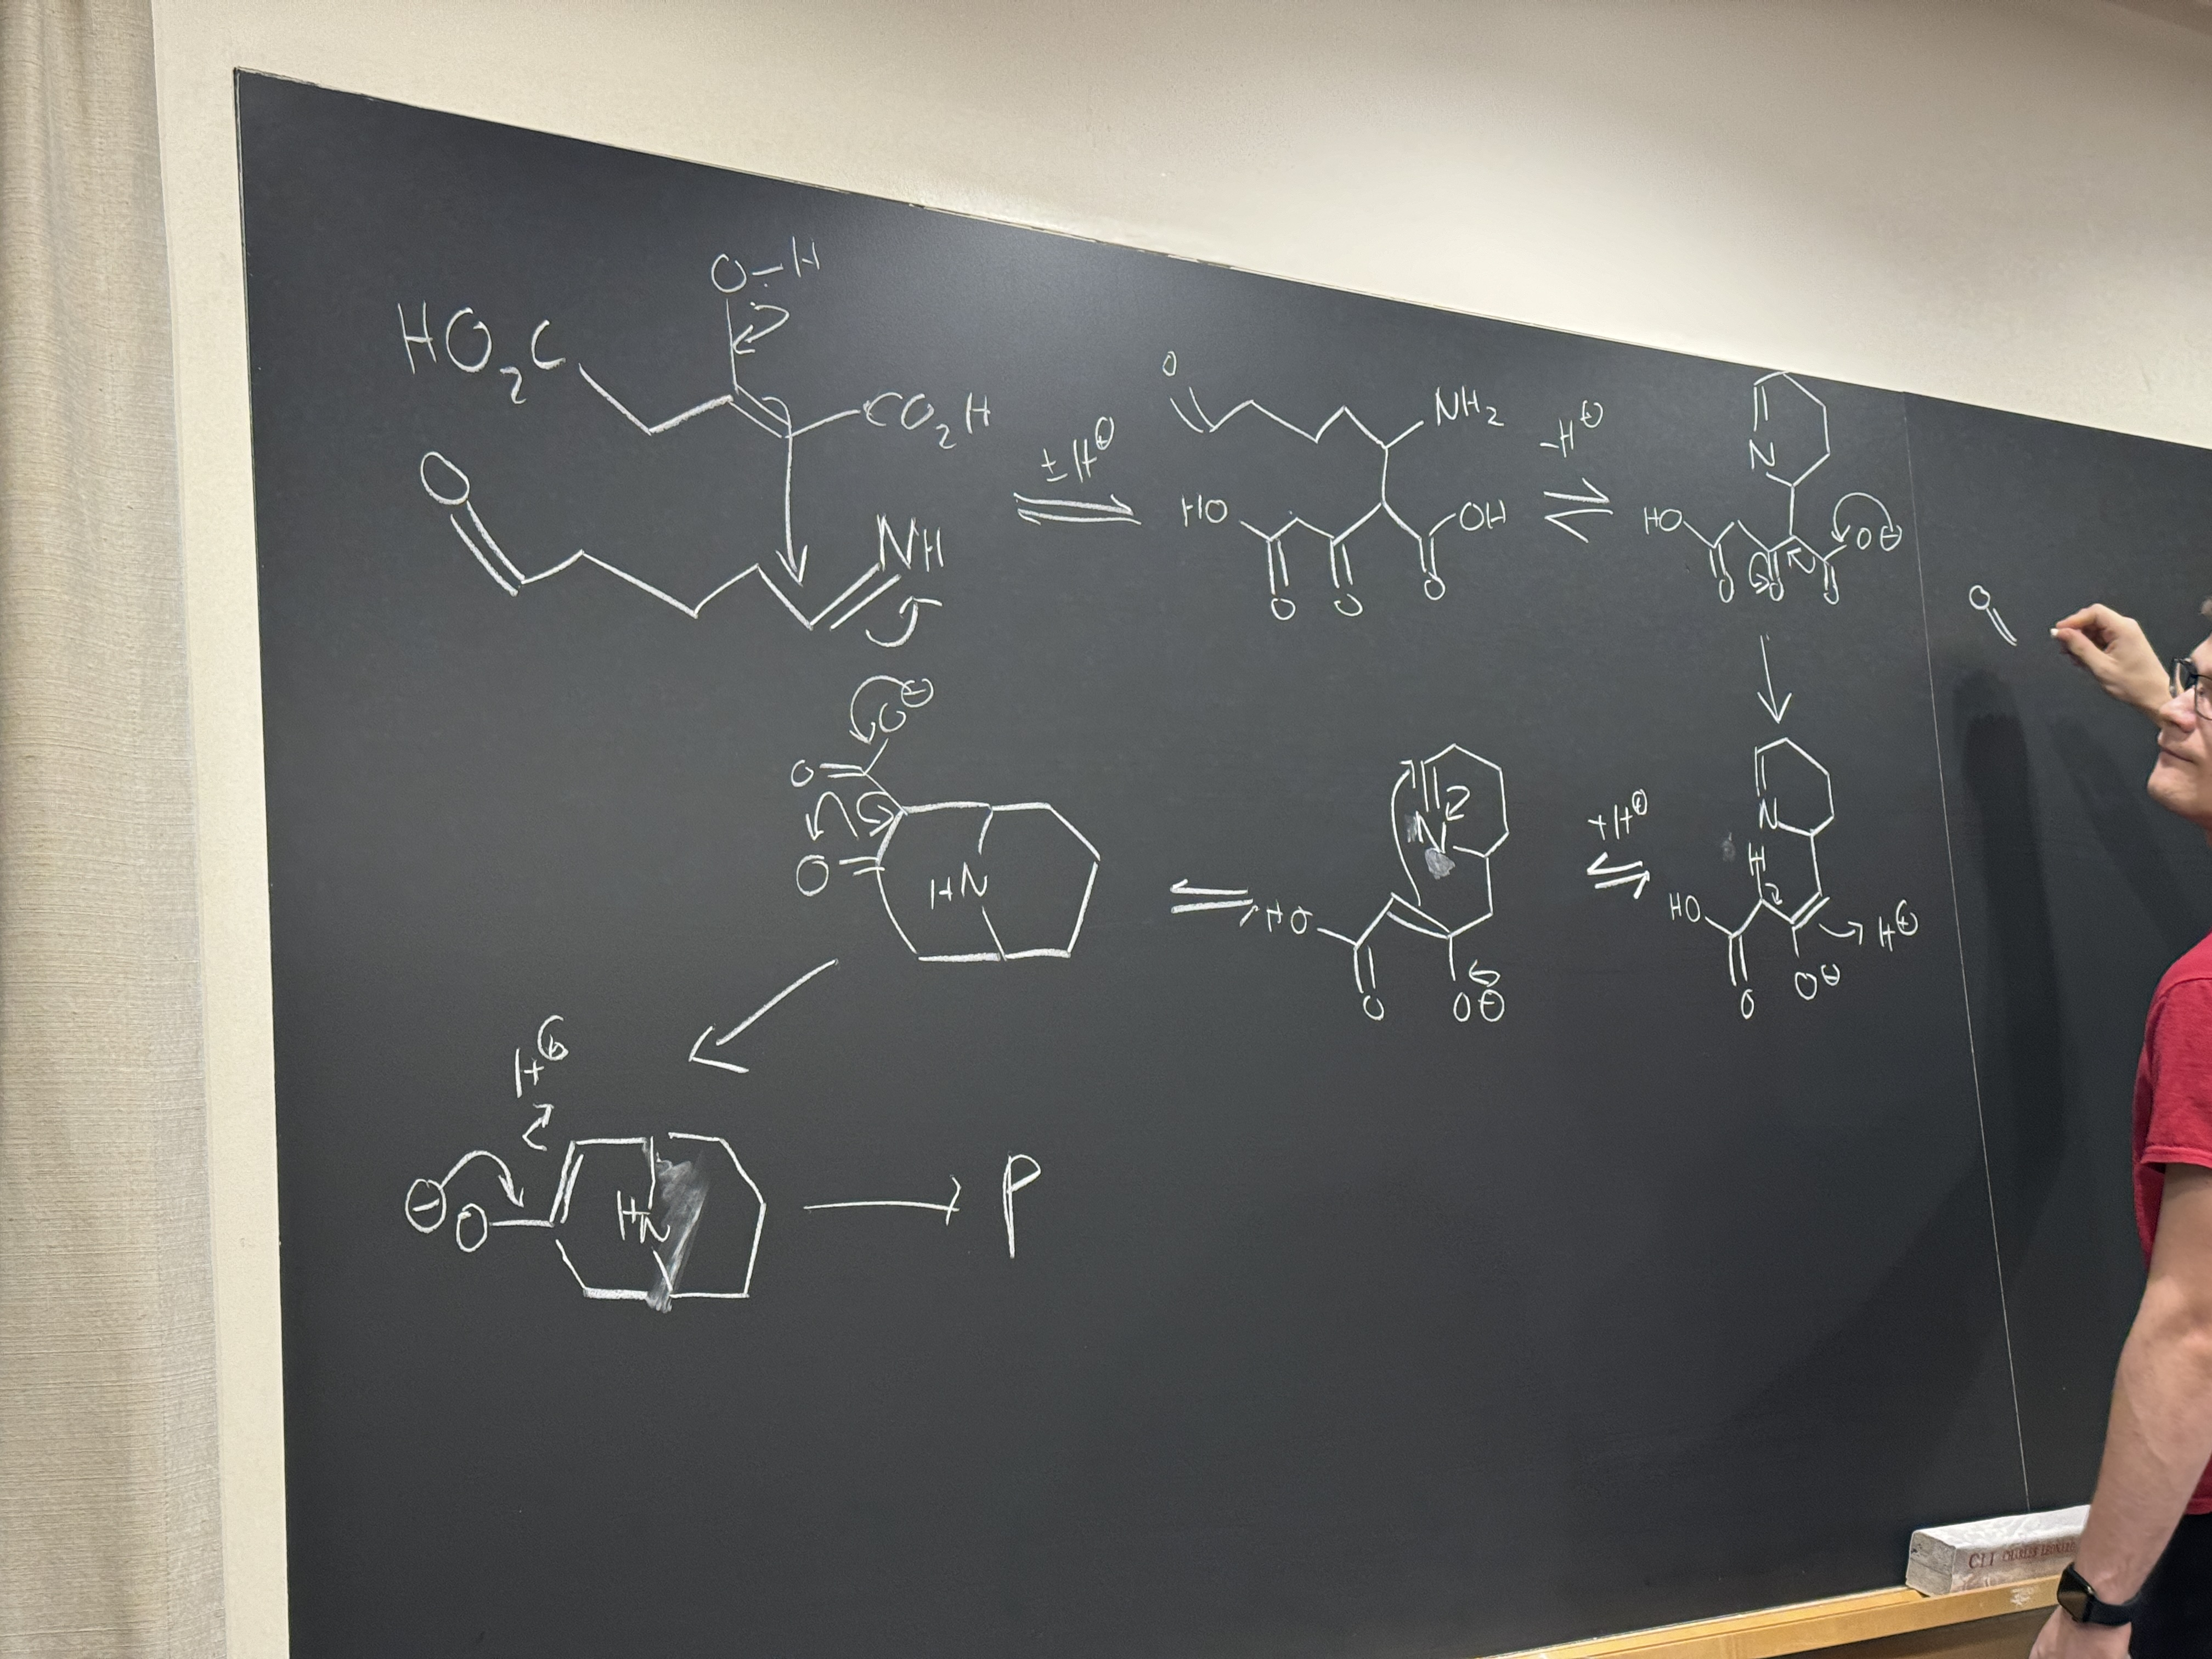
\includegraphics[width=0.8\linewidth]{WPSet1Q1S.JPG}
        \caption{Wendlandt PSet 1, Q1 solution.}
        \label{fig:WPSet1Q1S}
    \end{figure}
    \pagebreak
    \item We now begin discussing Problem 4.
    \begin{figure}[h!]
        \centering
        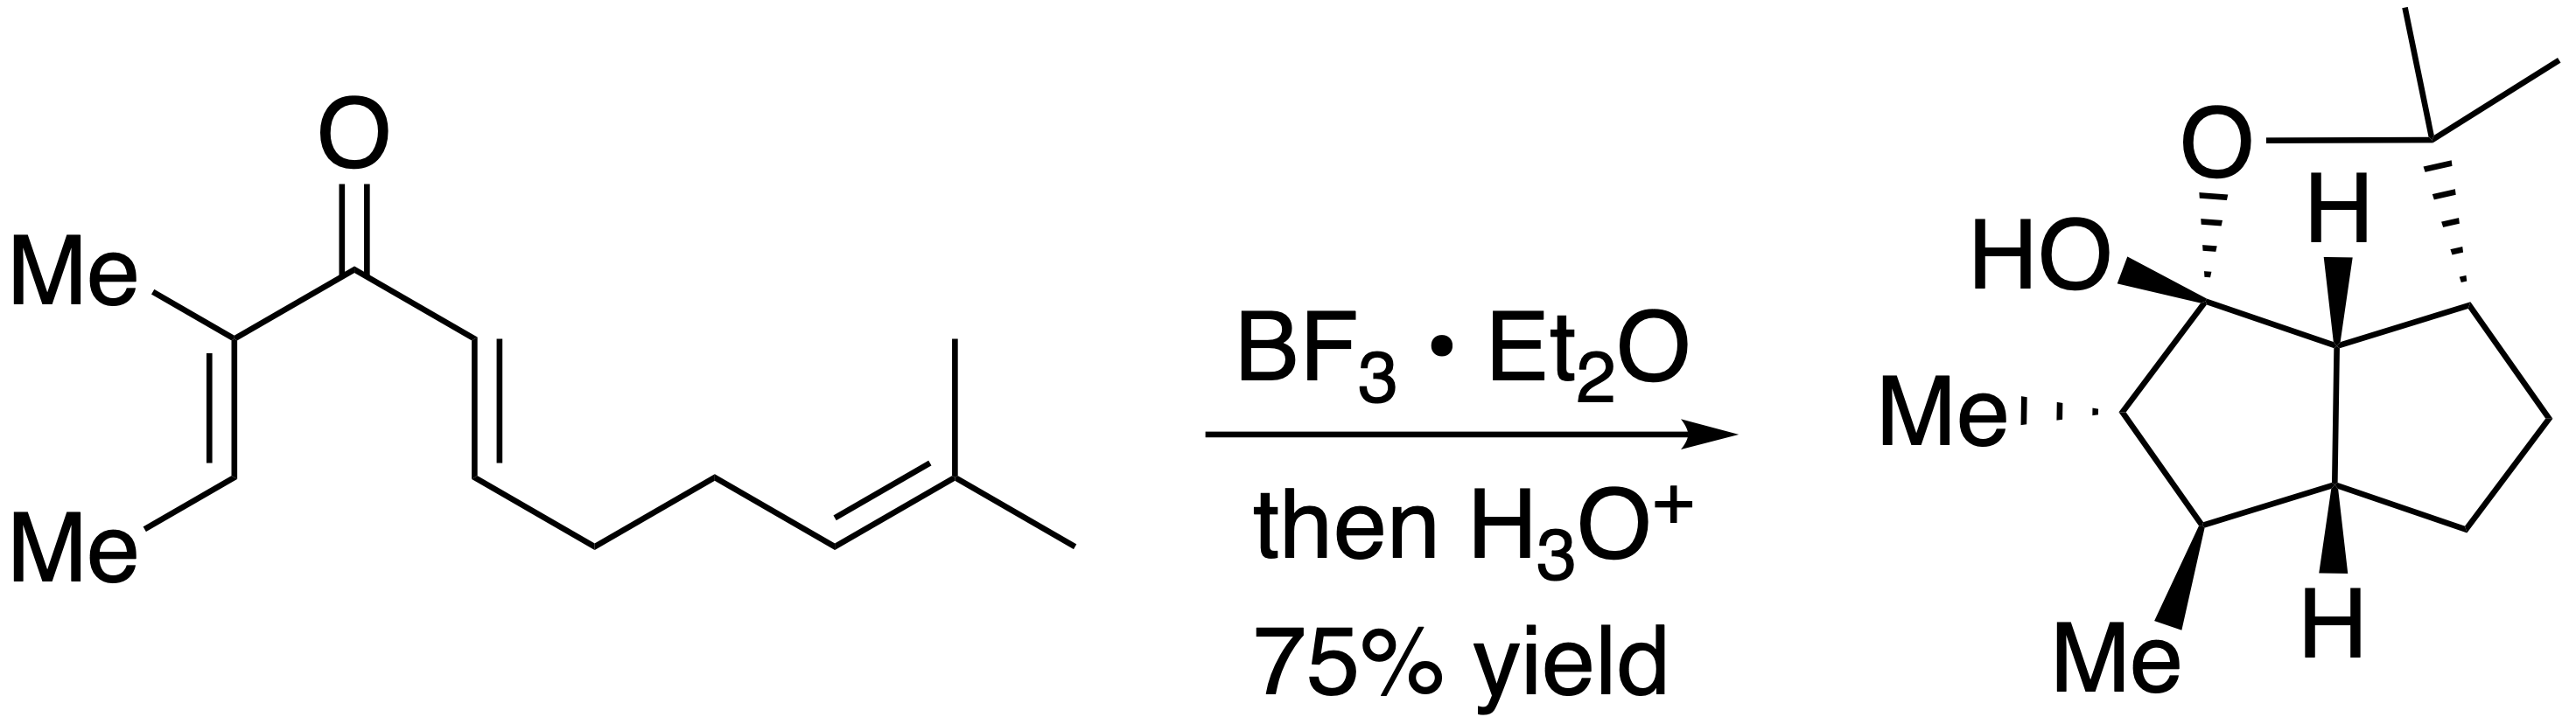
\includegraphics[width=0.45\linewidth]{WPSet1Q4.png}
        \caption{Wendlandt PSet 1, Q4.}
        \label{fig:WPSet1Q4}
    \end{figure}
    \item This is a \textbf{Nazarov reaction}, which is covered in Clayden.
    \item The initial electrocyclization is conrotatory; we need a continuous sequence of $\pi$-orbitals to get this.
    \item The Nazarov is a very powerful tool for making 5-membered rings, but the cation that it leaves oblates a ton of the stereochemical information.
    \item \textbf{Torquoselective reaction}: ...
    \item Orbital analysis yields a structure with the stereochemistry that 
    \item 5,5-trans ring fusions aren't known outside of very unique synthetic constructs. The difference in energy is a huge $\SIrange{5}{7}{\kilo\calorie\per\mole}$.
    \item Scott Denmark has developed strong Lewis acid activation of strong Lewis bases.
    \begin{itemize}
        \item Thus, from the perspective of both the activated Lewis base heteroatom and the perspective of the carbocation, this \ce{C-O} bond-forming reaction should proceed before the acid workup.
    \end{itemize}
    \item Whenever you see a cycloaddition, start thinking about the orbital structure of the HOMO and LUMO.
    \item Altogether, the full solution to PSet 1, Q4 is on the next page.
    \begin{figure}[H]
        \centering
        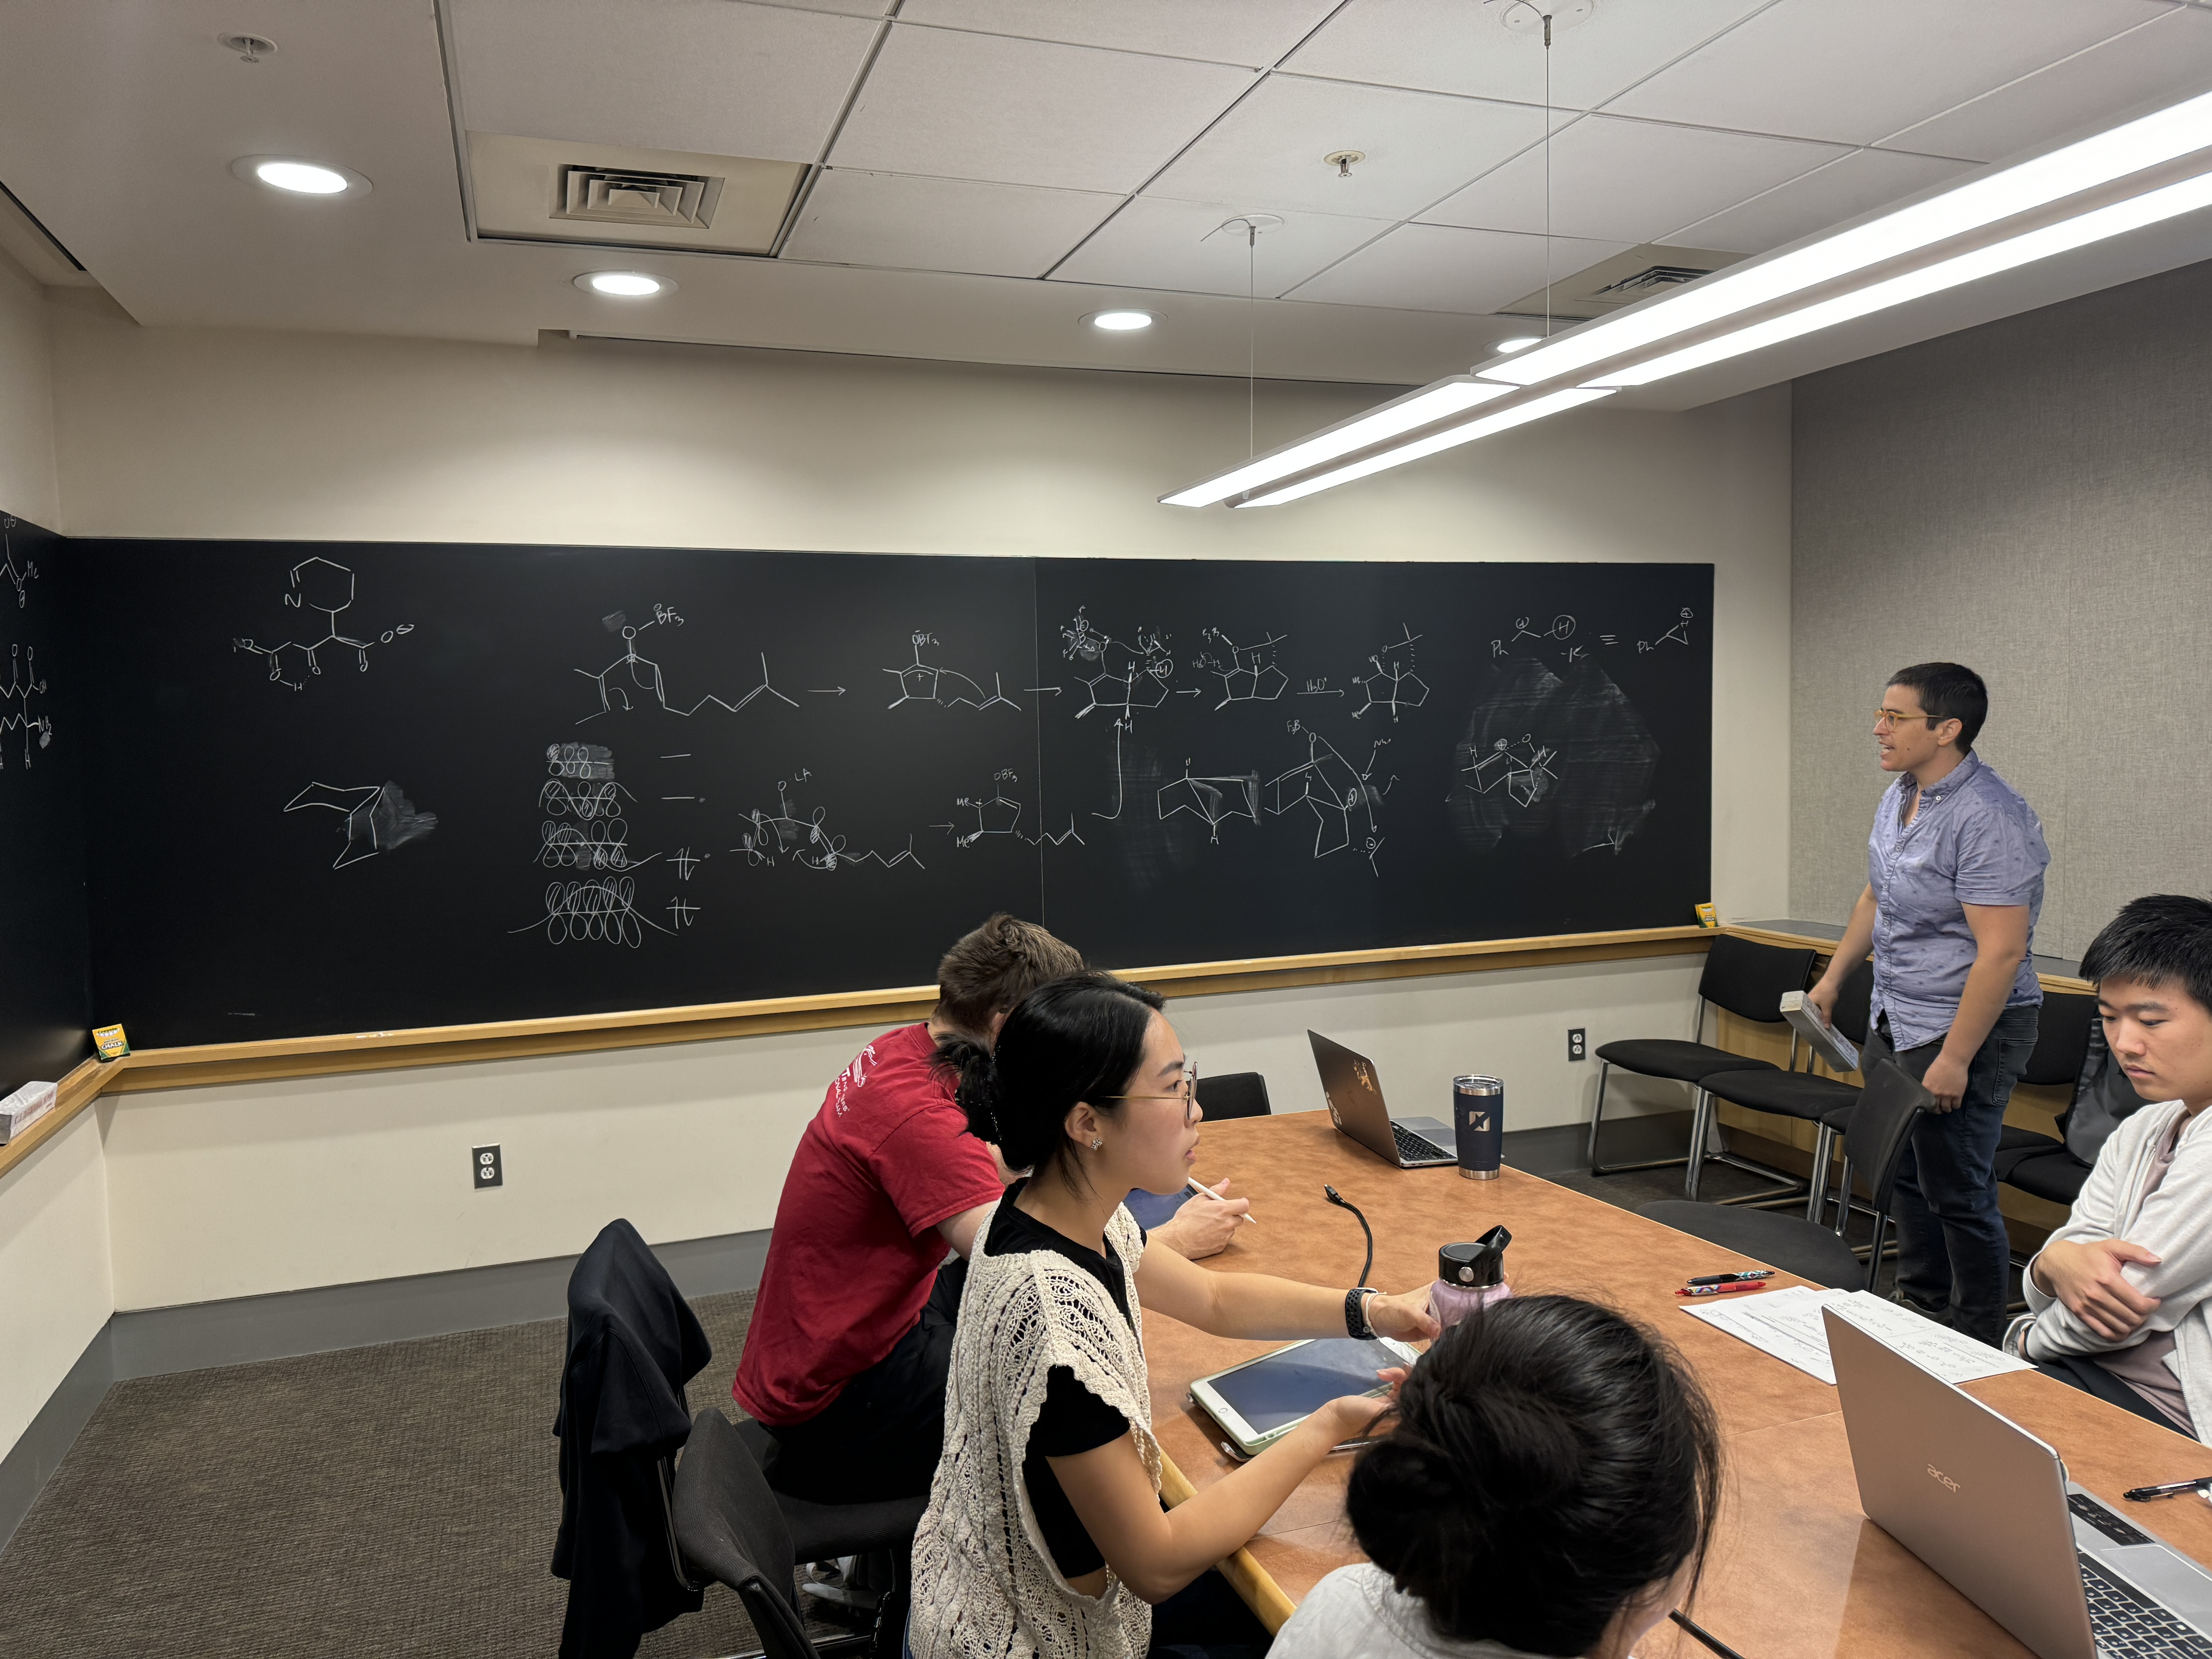
\includegraphics[width=0.8\linewidth]{WPSet1Q4S.JPG}
        \caption{Wendlandt PSet 1, Q4 solution.}
        \label{fig:WPSet1Q4S}
    \end{figure}
    \pagebreak
    \item We now begin discussing Problem 8.
    \begin{figure}[h!]
        \centering
        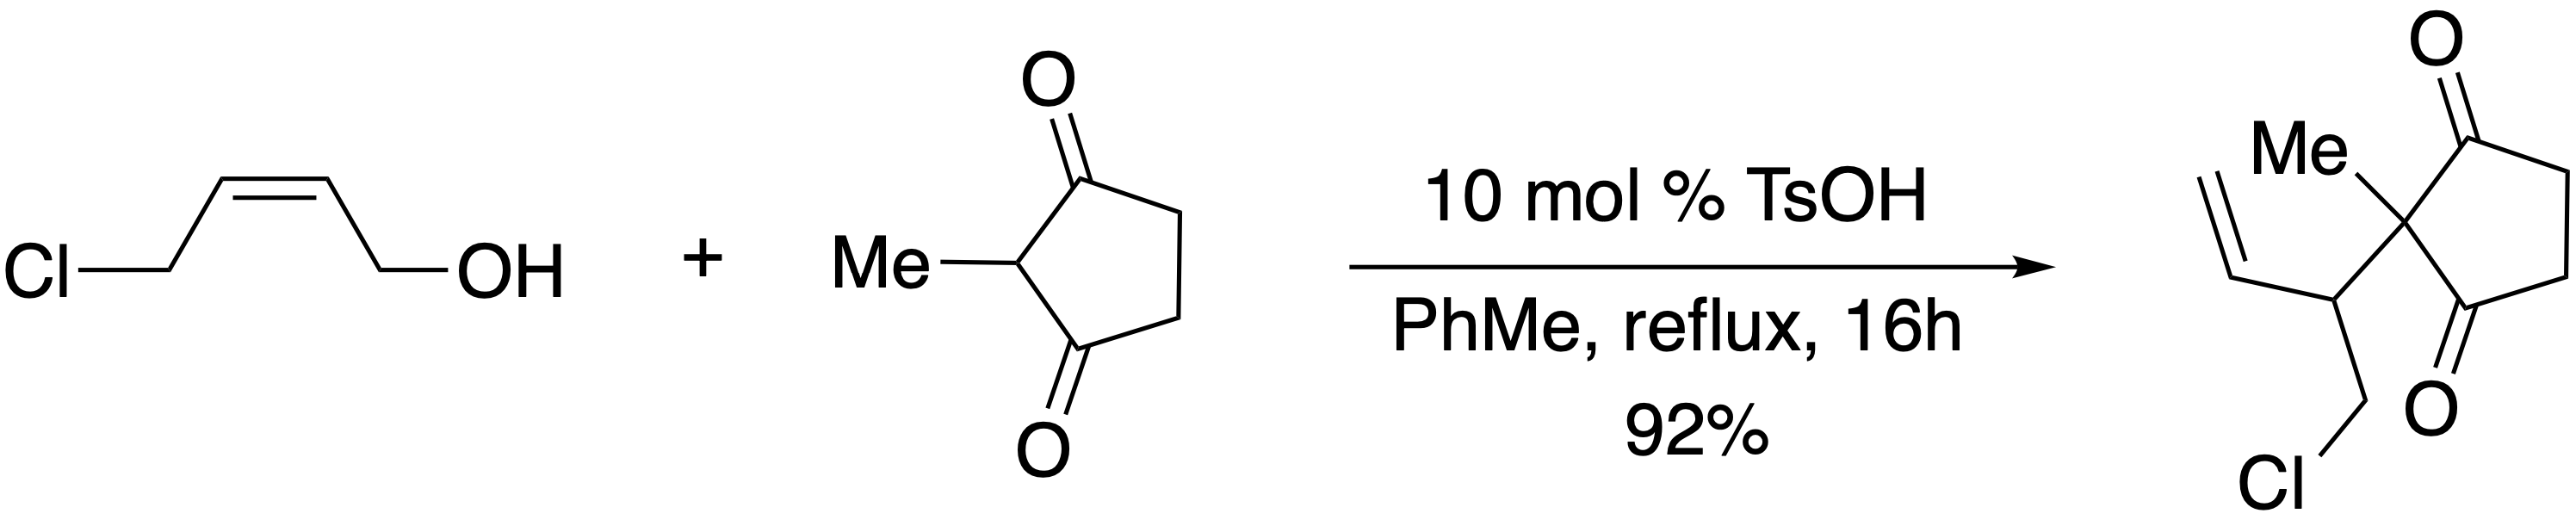
\includegraphics[width=0.6\linewidth]{WPSet1Q8.png}
        \caption{Wendlandt PSet 1, Q8.}
        \label{fig:WPSet1Q8}
    \end{figure}
    \item The thing I proposed is called an S\textsubscript{N}2' reaction, i.e., the attack of one species not on the leaving group but on the conjugated position a couple of carbons away.
    \begin{itemize}
        \item My mechanism is \emph{plausible} but not \emph{defensible}.
        \item The \ce{OH} is not the most Lewis basic species in solution.
    \end{itemize}
    \item Protonating a hemiacetal will be easier than Frank's proposition of protonating the alcohol.
    \begin{itemize}
        \item Alison proposed 1,2-addition and 1,4-addition.
    \end{itemize}
    \item We end with a \textbf{Claisen rearrangement}.
    \item You get a \emph{stabilized} enol structure. Enol is better than enolate for acidic solution.
    \item You use the nucleophilic part to rearrange the electrophilic part.
    \item Altogether, the full solution to PSet 1, Q8 is on the next page.
    \begin{figure}[h!]
        \centering
        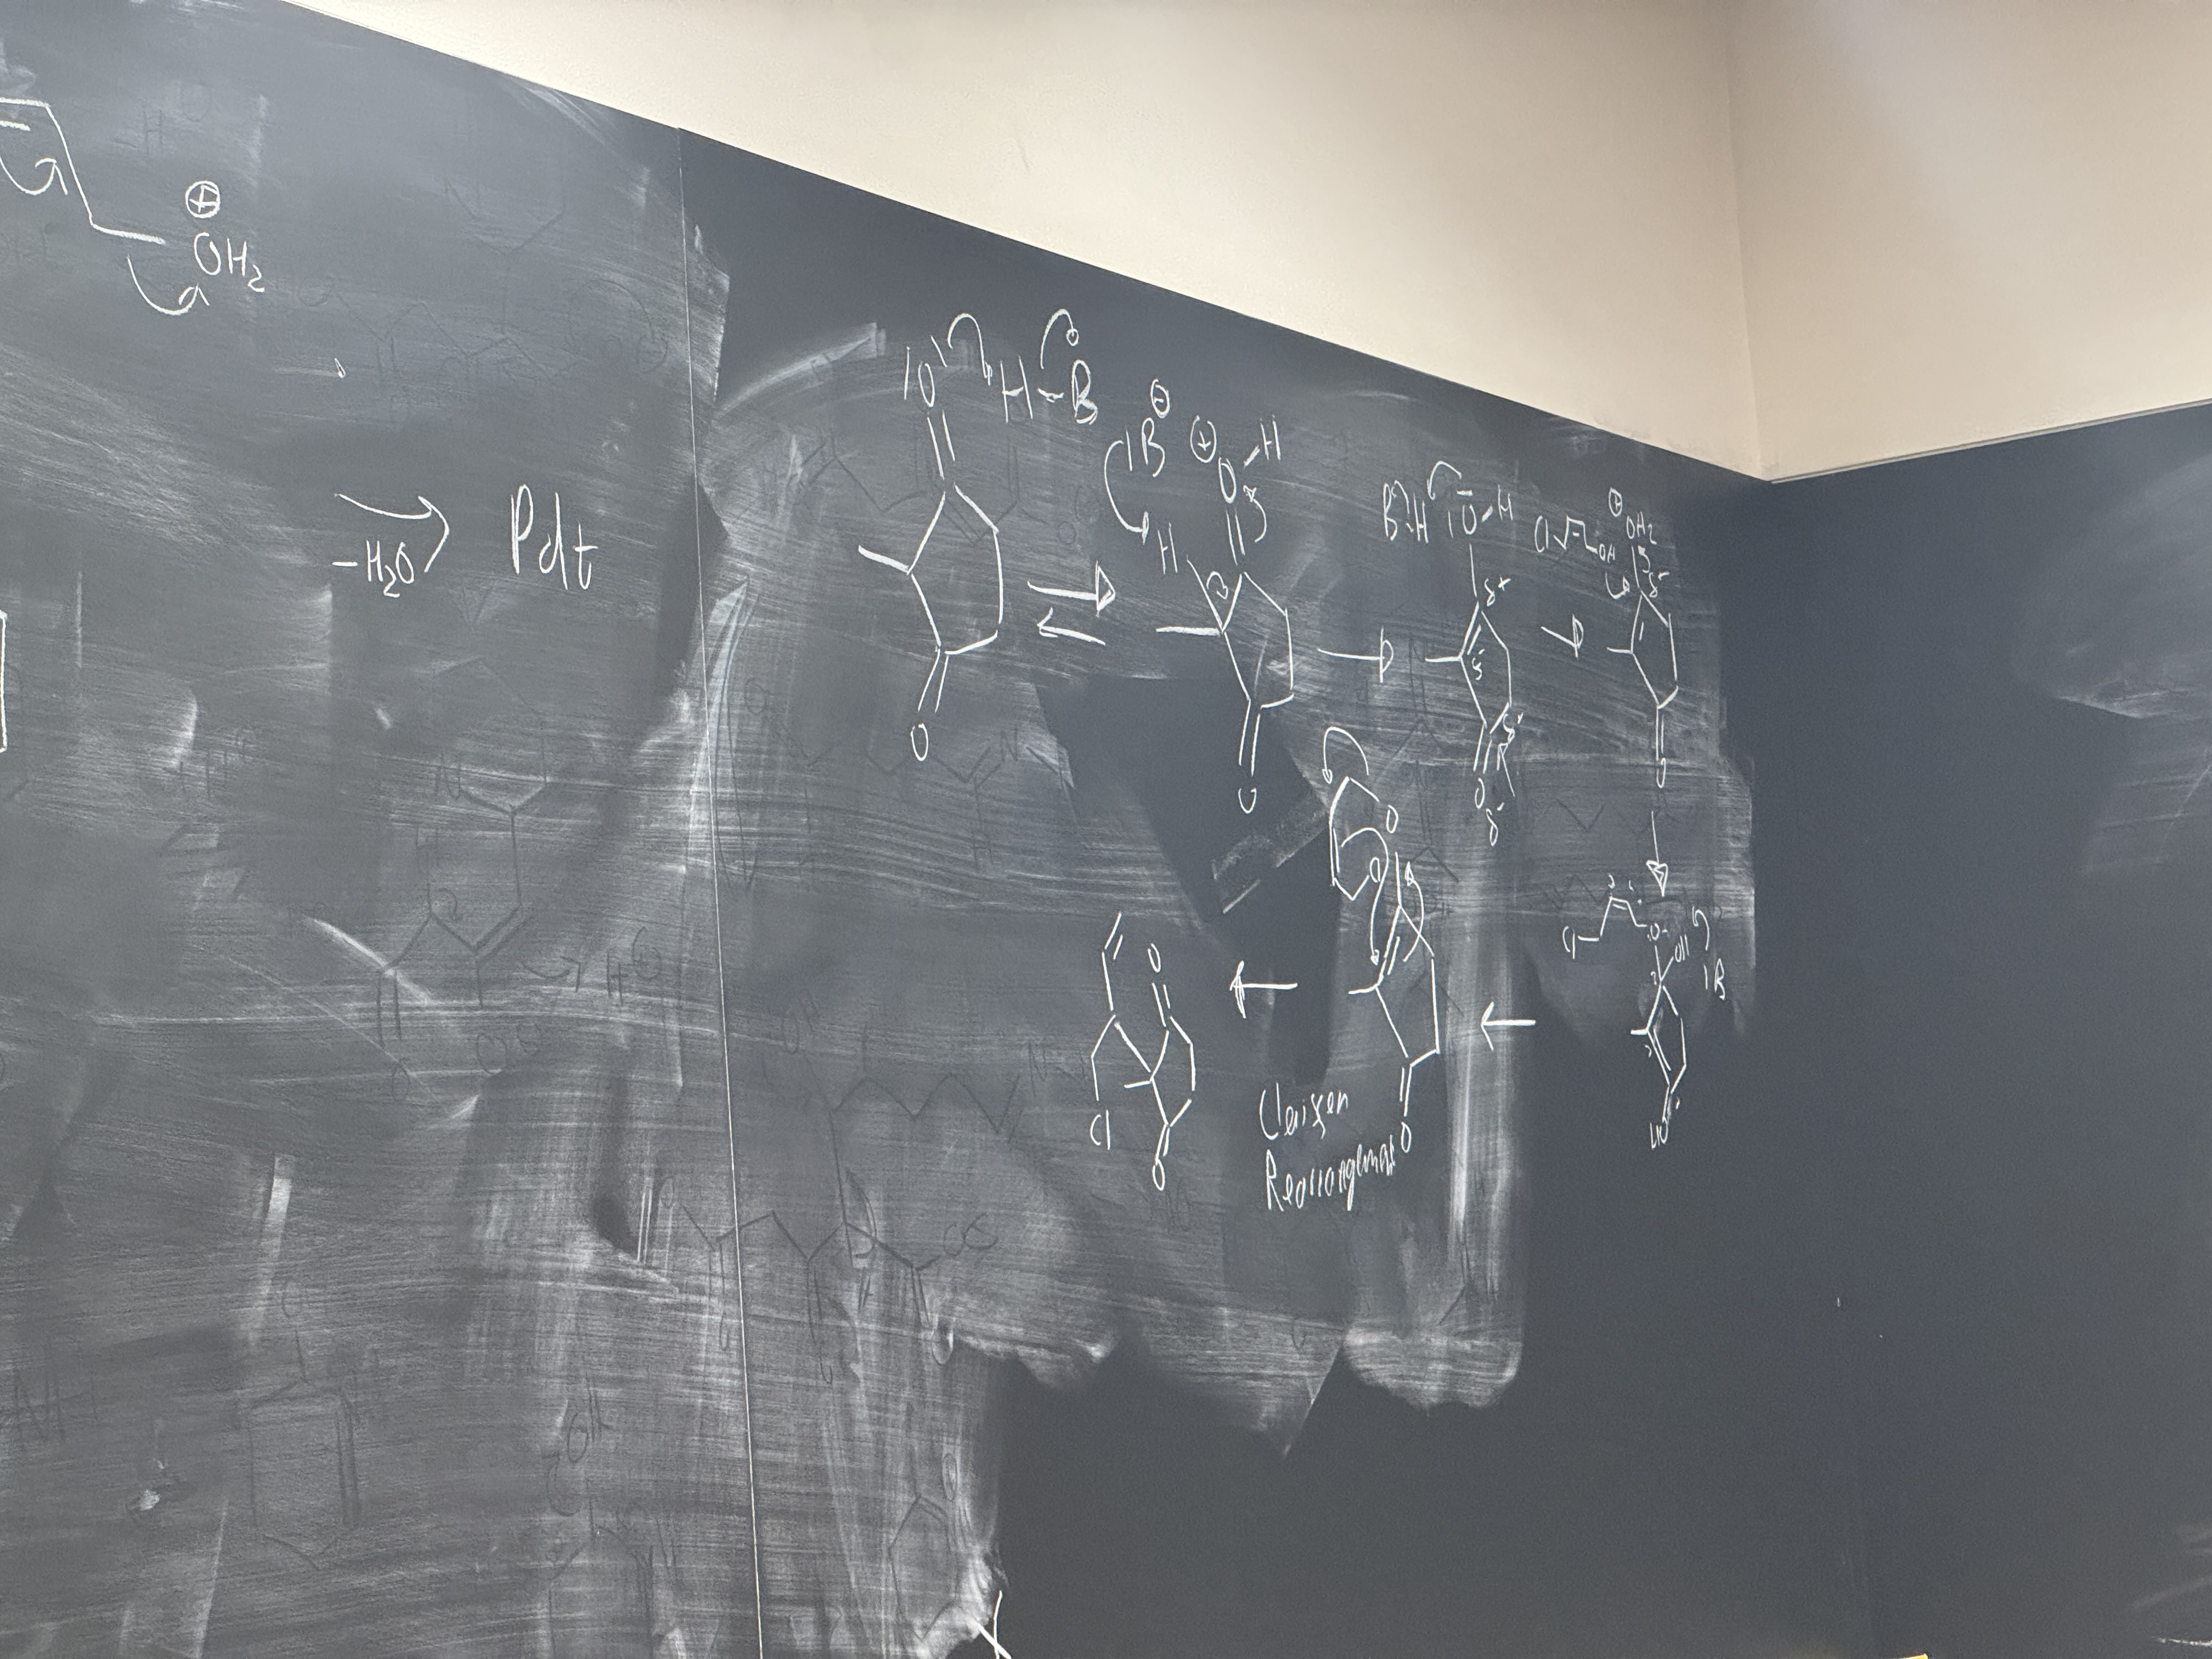
\includegraphics[width=0.8\linewidth]{WPSet1Q8S.JPG}
        \caption{Wendlandt PSet 1, Q8 solution.}
        \label{fig:WPSet1Q8S}
    \end{figure}
\end{itemize}



\section{Problems 3, 5, 6, and 7}
\begin{itemize}
    \item \marginnote{9/18:}Alison used to play ice hockey!
    \item We now begin discussing Problem 6.
    \begin{figure}[h!]
        \centering
        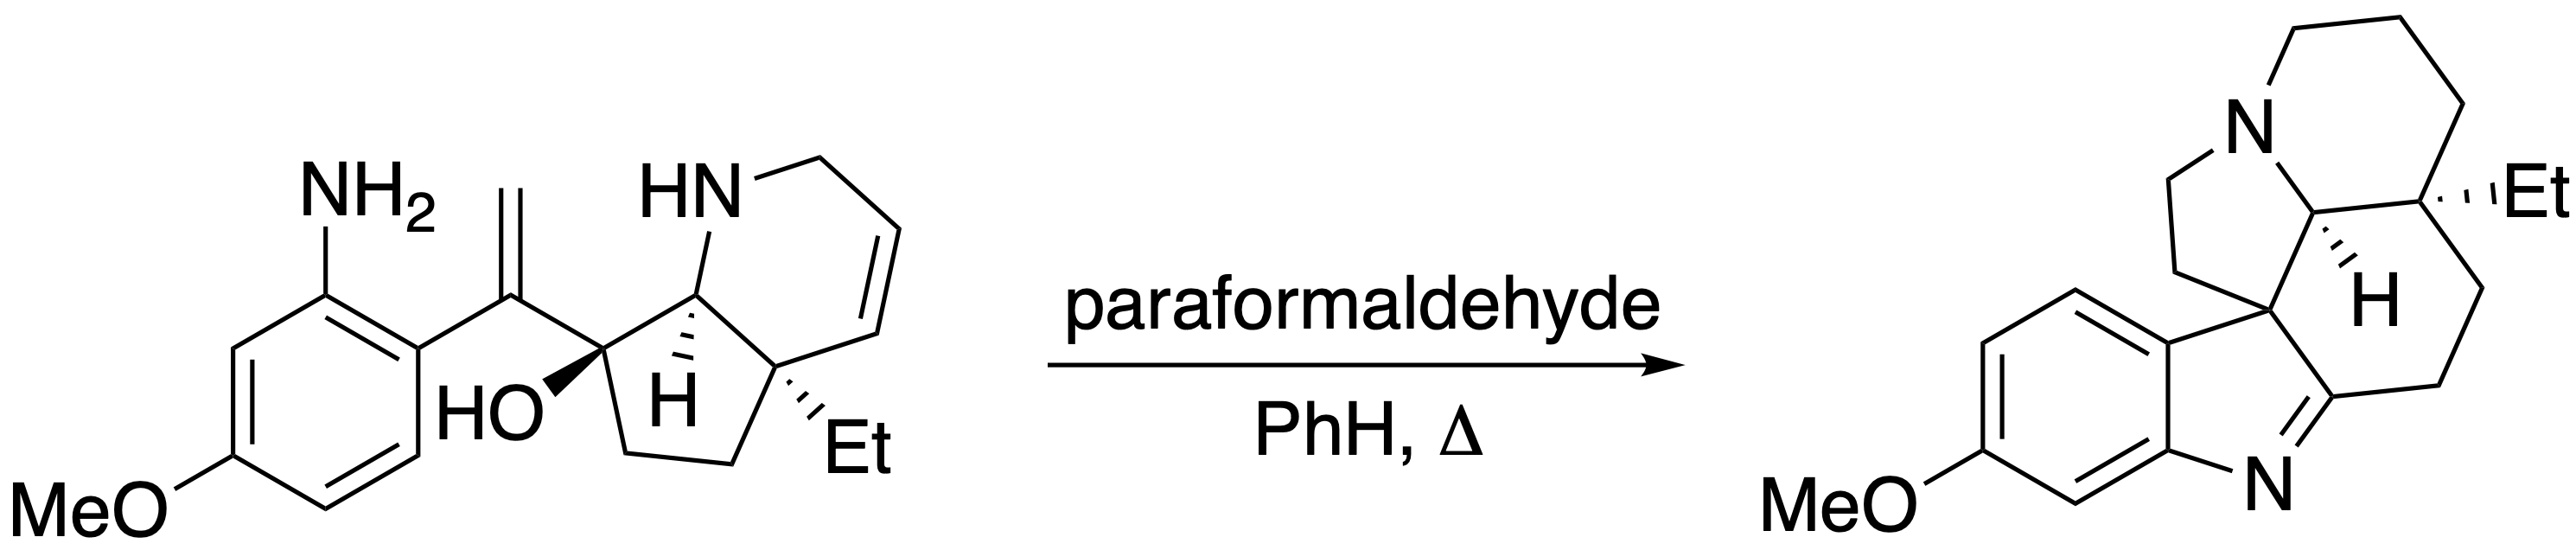
\includegraphics[width=0.6\linewidth]{WPSet1Q6.png}
        \caption{Wendlandt PSet 1, Q6.}
        \label{fig:WPSet1Q6}
    \end{figure}
    \begin{itemize}
        \item I was the only person to have an idea for 6!
        \item There was a typo in the PSet.
    \end{itemize}
    \item \textbf{Sigmatropic step}.
    \begin{itemize}
        \item The $sp^3$ hybrid orbitals become $p$'s. At some point in the transition state, they look $p$-like enough.
        \item It will be \textbf{conrotatory}, so fake substitutents come out on the same side.
        \item Don't remember the rules; just draw the orbitals and figure it out.
        \item David's pneumonic: 64 disco: 6 disrotatory, 4 conrotatory. Then for light, you just reverse it.
    \end{itemize}
    \item Does everything happen very quickly, or do things pull apart first and we tautomerize to a ketone before we go back to an enol and react.
    \item Nonpolar solvent and high temperature often implies pericyclic reaction!
    \item Where are acids and bases coming from? The molecule itself? How does the condensation occur?
    \begin{itemize}
        \item Protonated piperidine: $\pKa=10$.
        \item Protonated aniline: $\pKa=8$.
        \item Learn the \href{http://ccc.chem.pitt.edu/wipf/MechOMs/evans_pKa_table.pdf}{Evans} $\pKa$ table!!
        \item The aniline probably forms the iminium with the formaldehyde, and that's just reversible until we can do the entropically favorable step.
    \end{itemize}
    \item Altogether, the full solution to PSet 1, Q6 is on the next page.
    \begin{figure}[H]
        \centering
        \begin{subfigure}[b]{\linewidth}
            \centering
            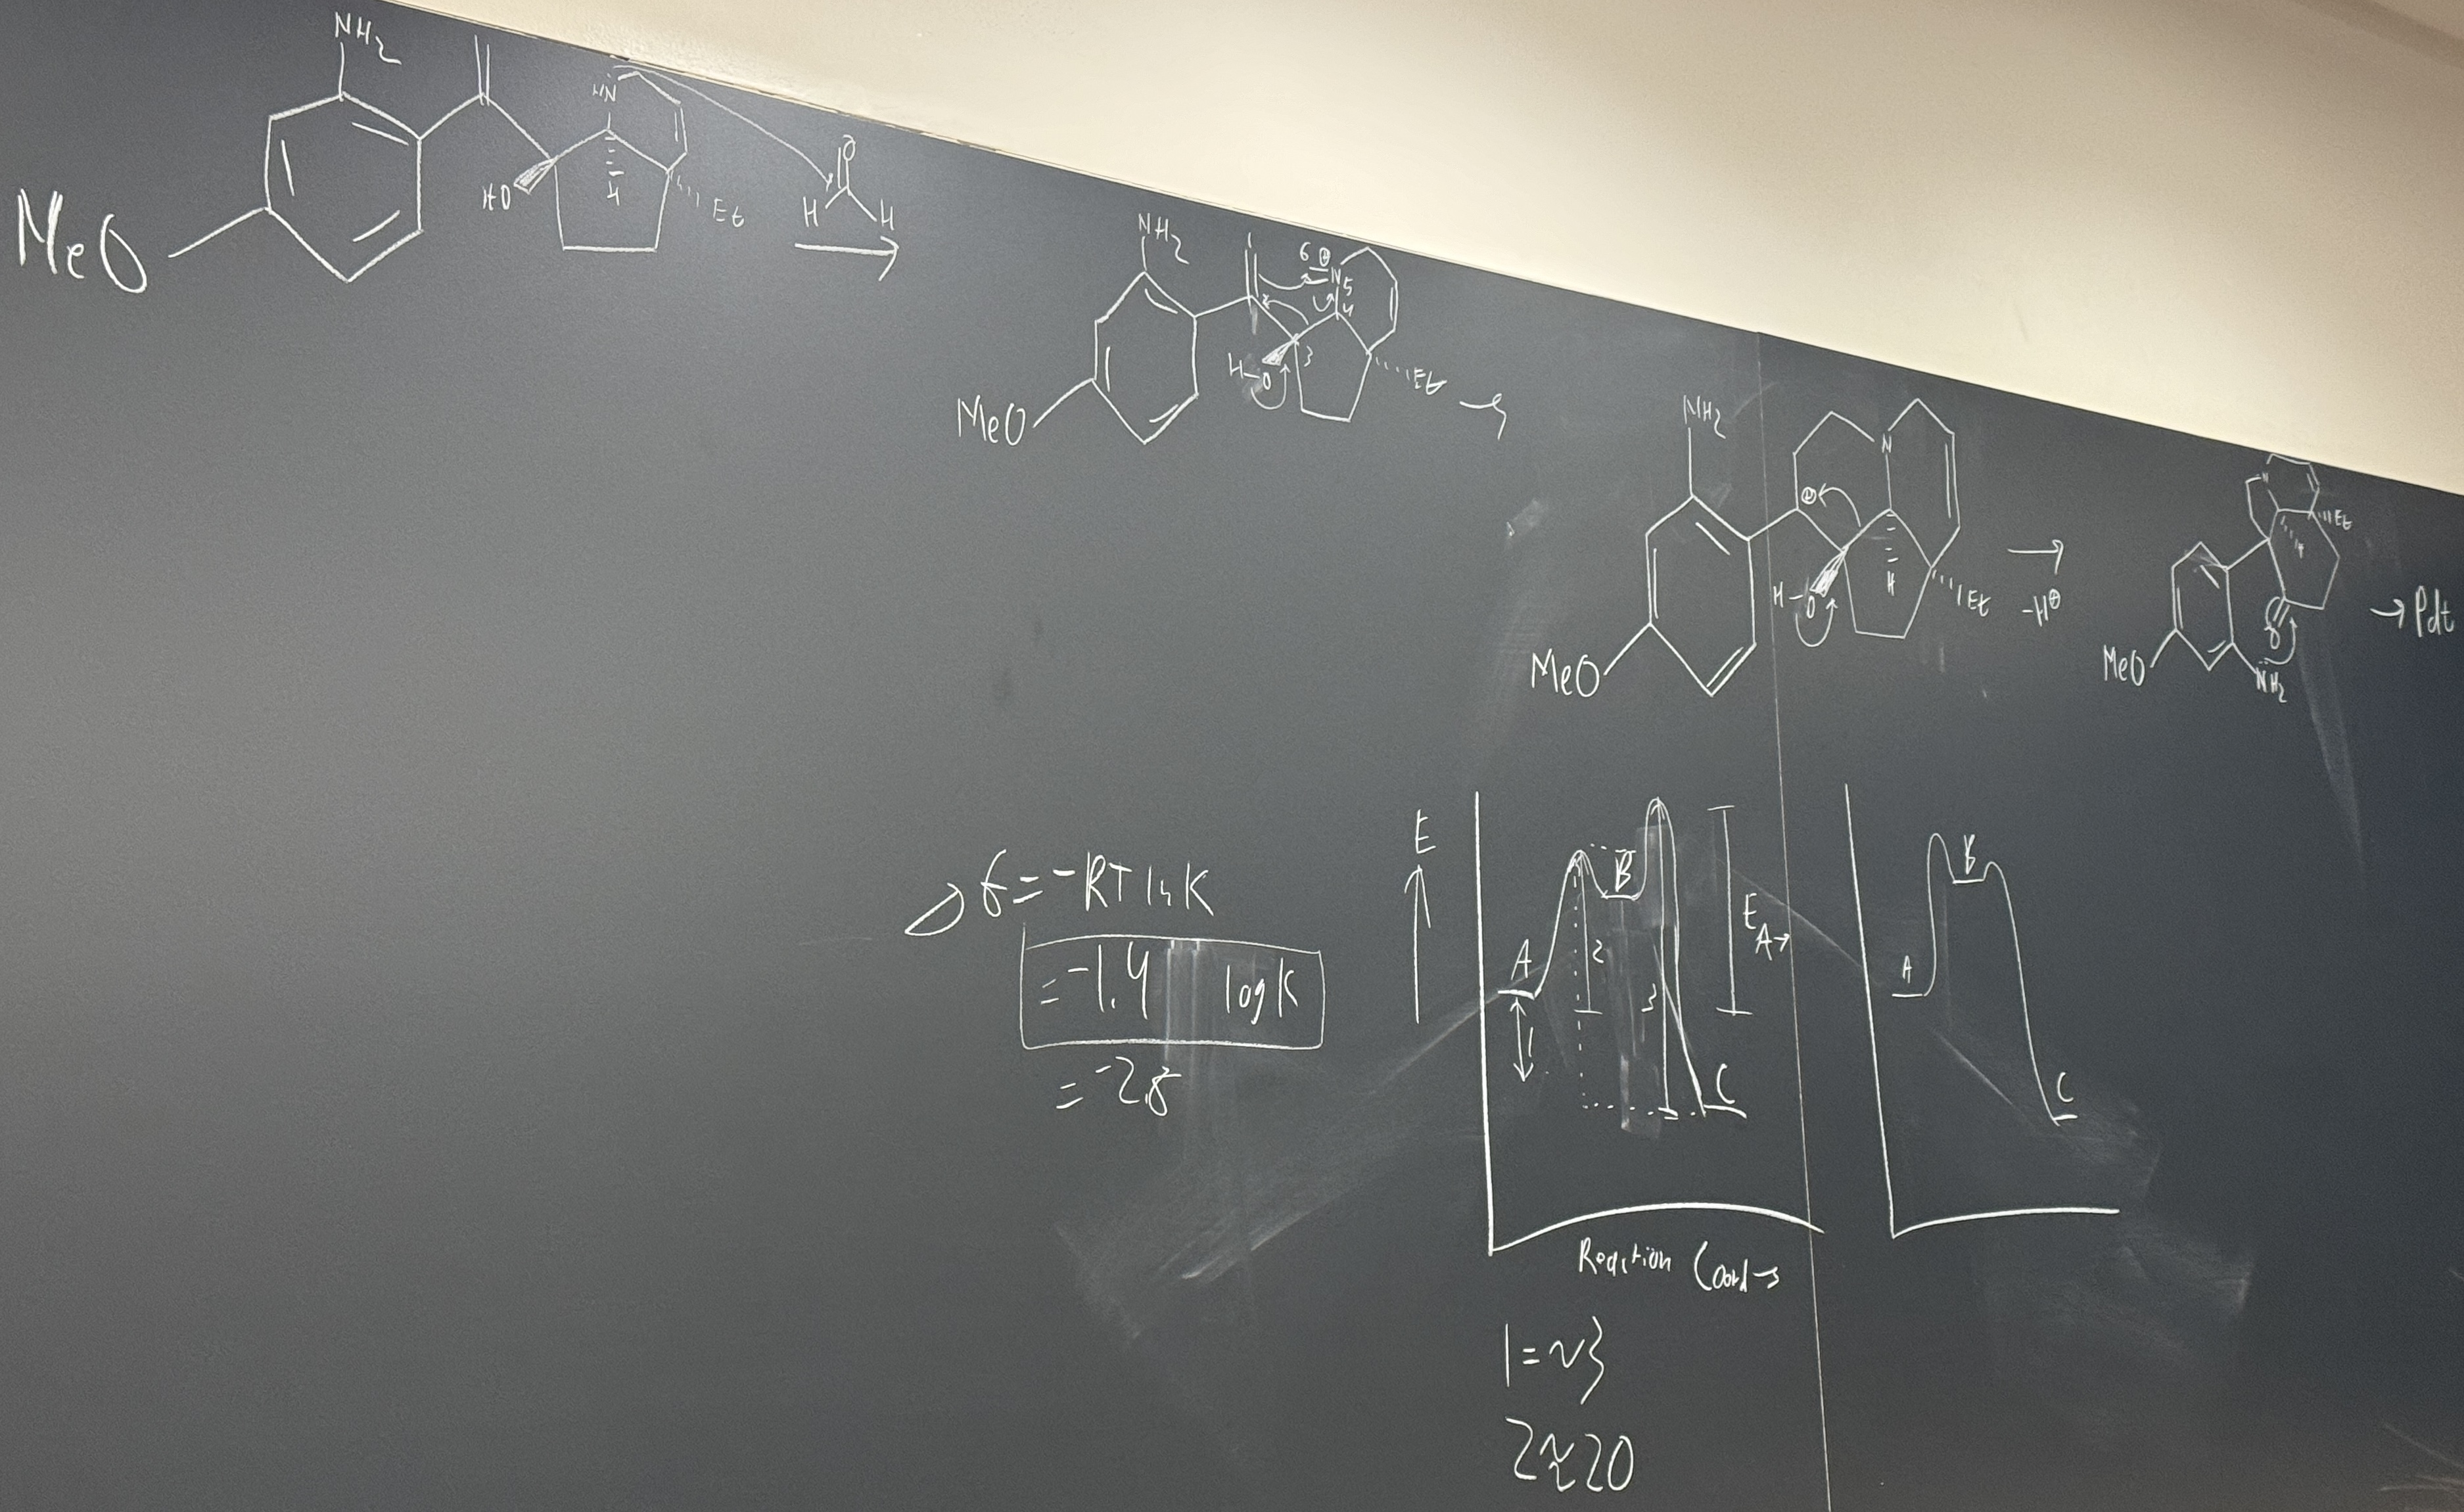
\includegraphics[width=0.8\linewidth]{WPSet1Q6Sa.JPG}
            \caption{My proposition.}
            \label{fig:WPSet1Q6Sa}
        \end{subfigure}\\[2em]
        \begin{subfigure}[b]{\linewidth}
            \centering
            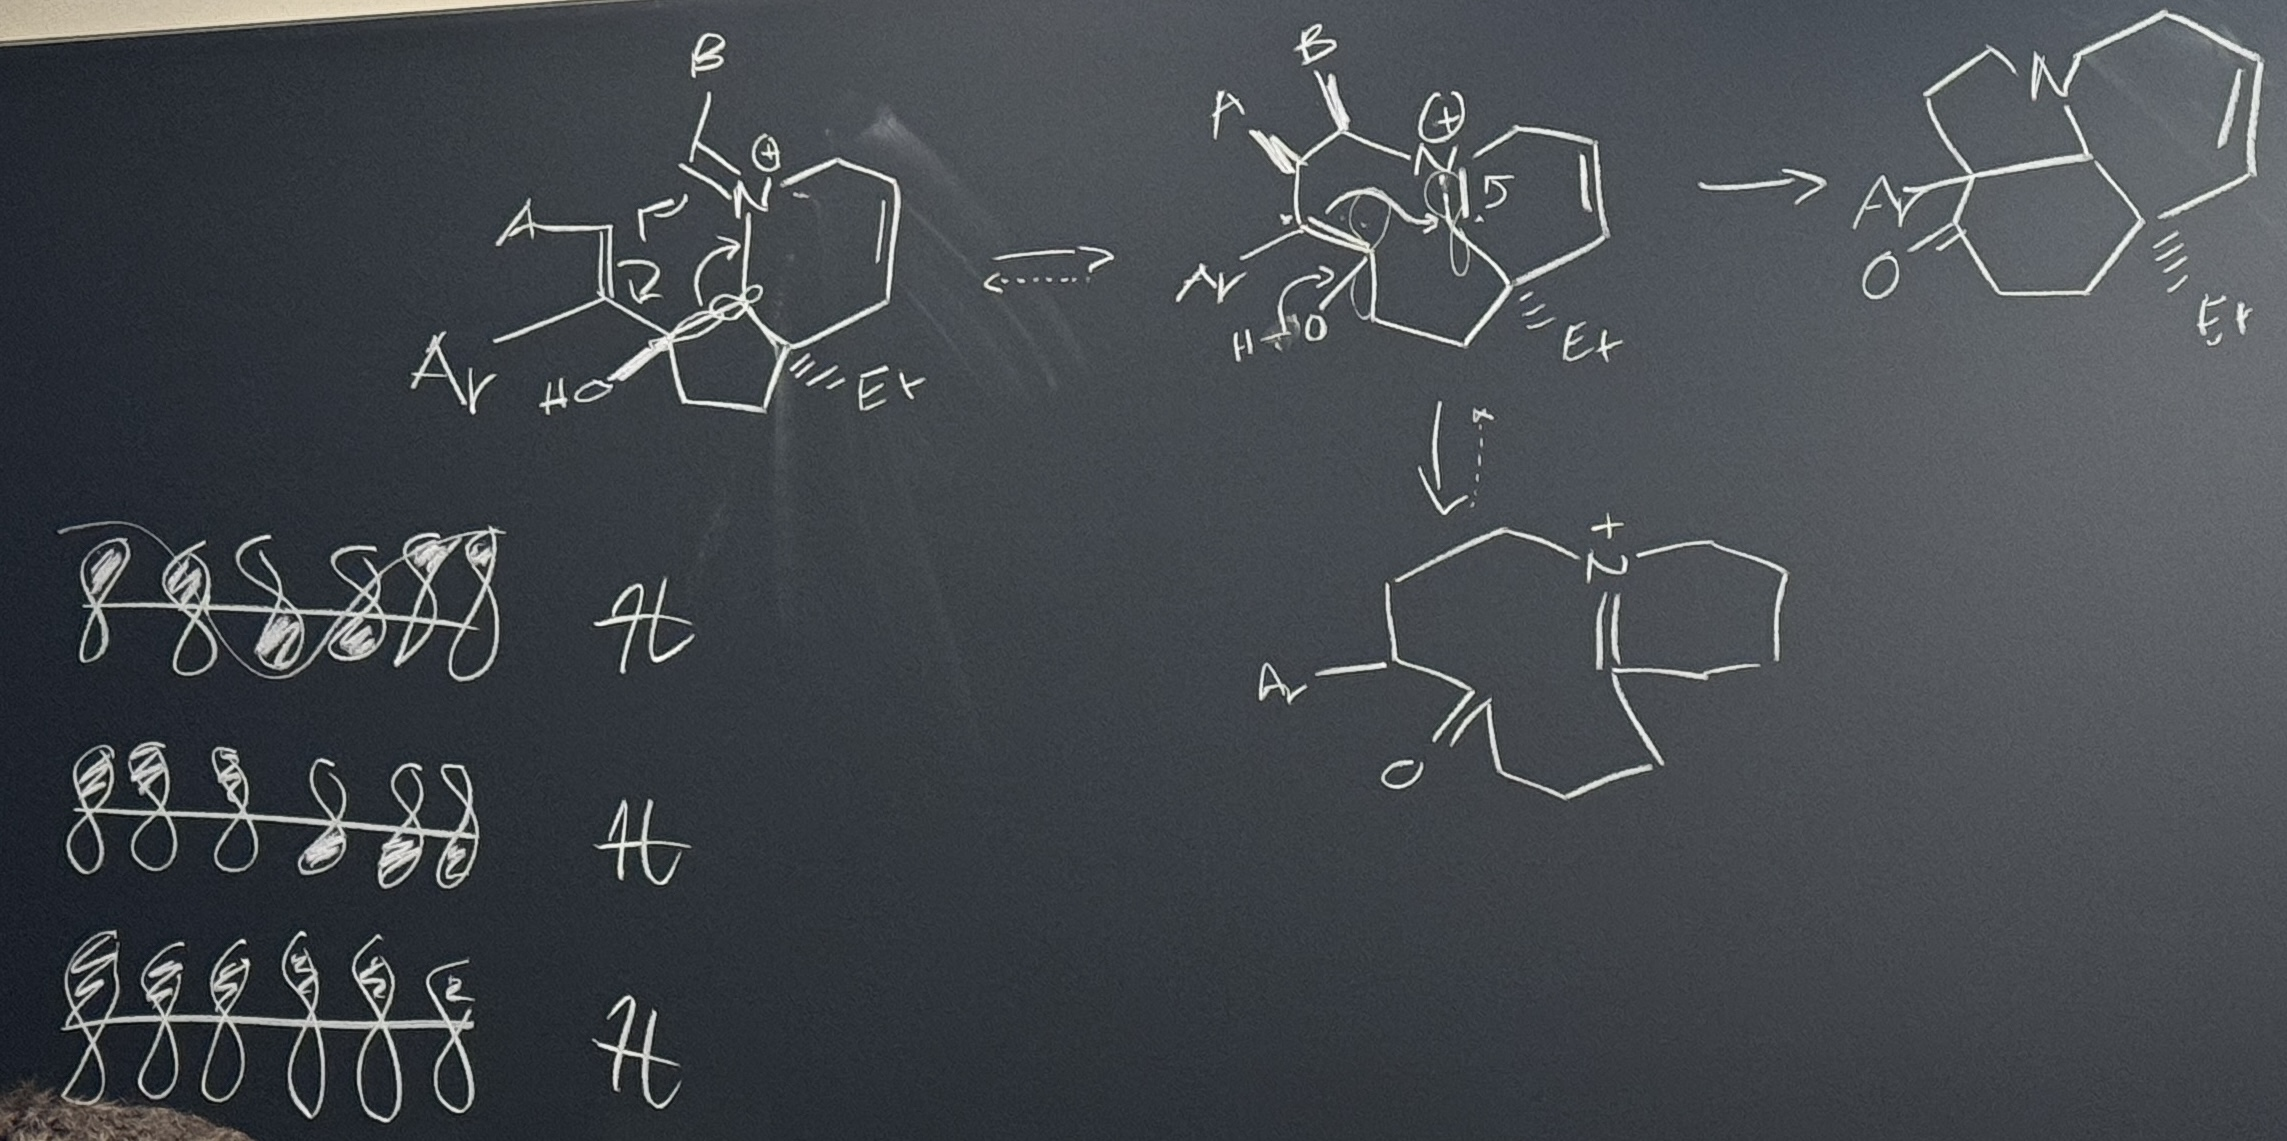
\includegraphics[width=0.8\linewidth]{WPSet1Q6Sb.JPG}
            \caption{Sigmatropic correction.}
            \label{fig:WPSet1Q6Sb}
        \end{subfigure}
        \caption{Wendlandt PSet 1, Q6 solution.}
        \label{fig:WPSet1Q6S}
    \end{figure}
    \pagebreak
    \item We now begin discussing Problem 7.
    \begin{figure}[h!]
        \centering
        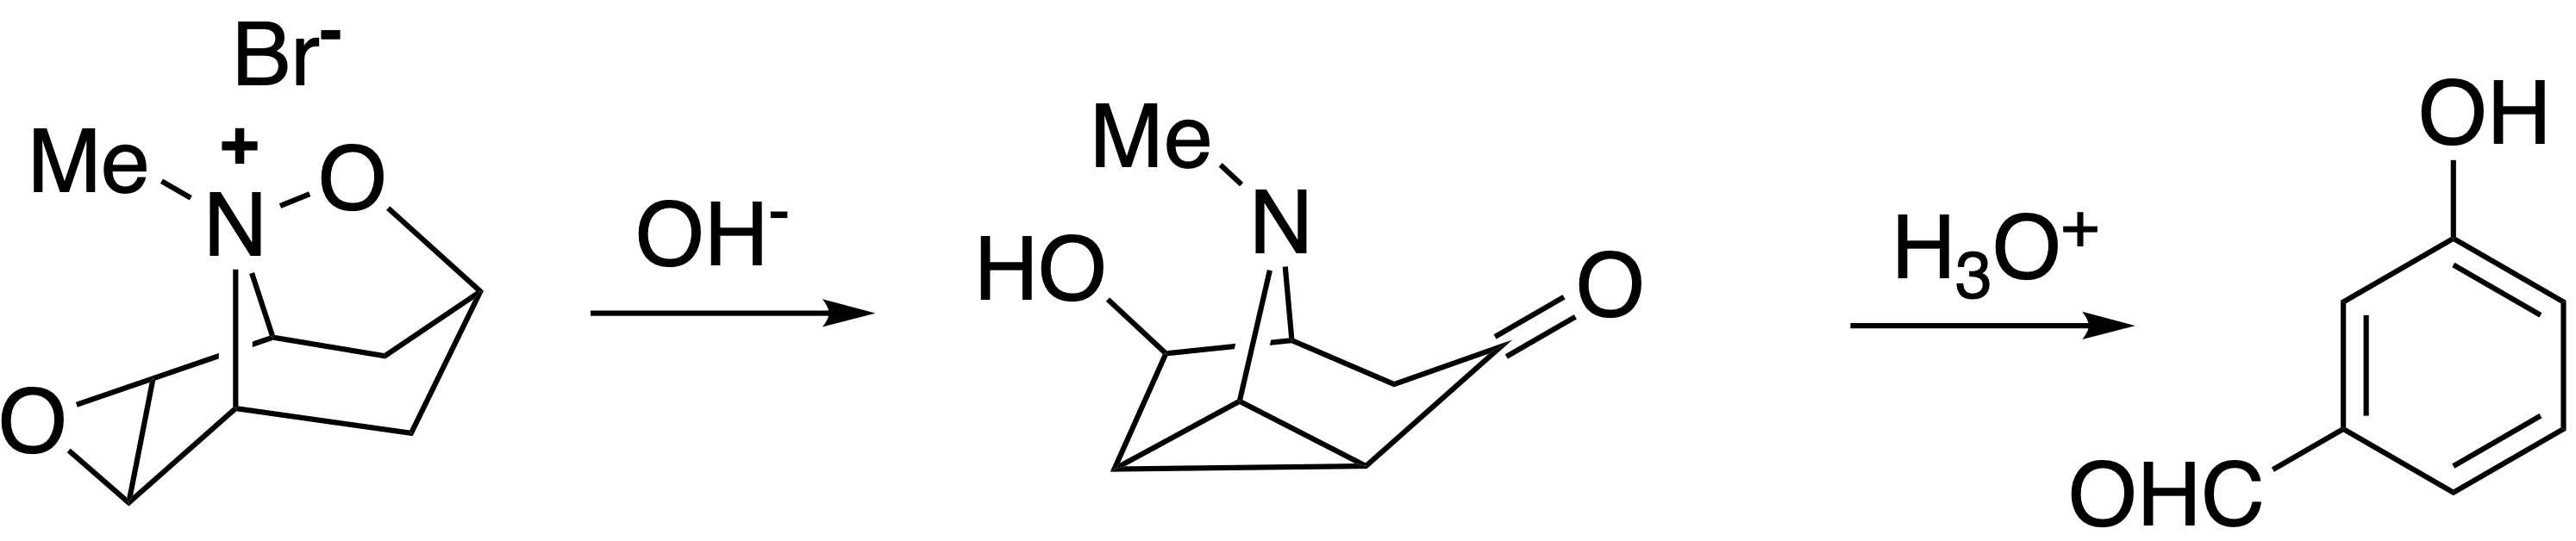
\includegraphics[width=0.5\linewidth]{WPSet1Q7.png}
        \caption{Wendlandt PSet 1, Q7.}
        \label{fig:WPSet1Q7}
    \end{figure}
    \item Somebody prepared a beautiful molecule, and then it just decomposed into this basic AF benzaldehyde derivative.
    \item This is probably a classic case of working in a lab, finding the decomposition product, going back to your PI, and then having to resort to arrow pushing to figure out what happened.
    \item The first step is helped by an antiperiplanar arrangement and the fact that the iminium wants its electron pair back.
    \item Altogether, the full solution to PSet 1, 7 is on the next page.
    \begin{figure}[h!]
        \centering
        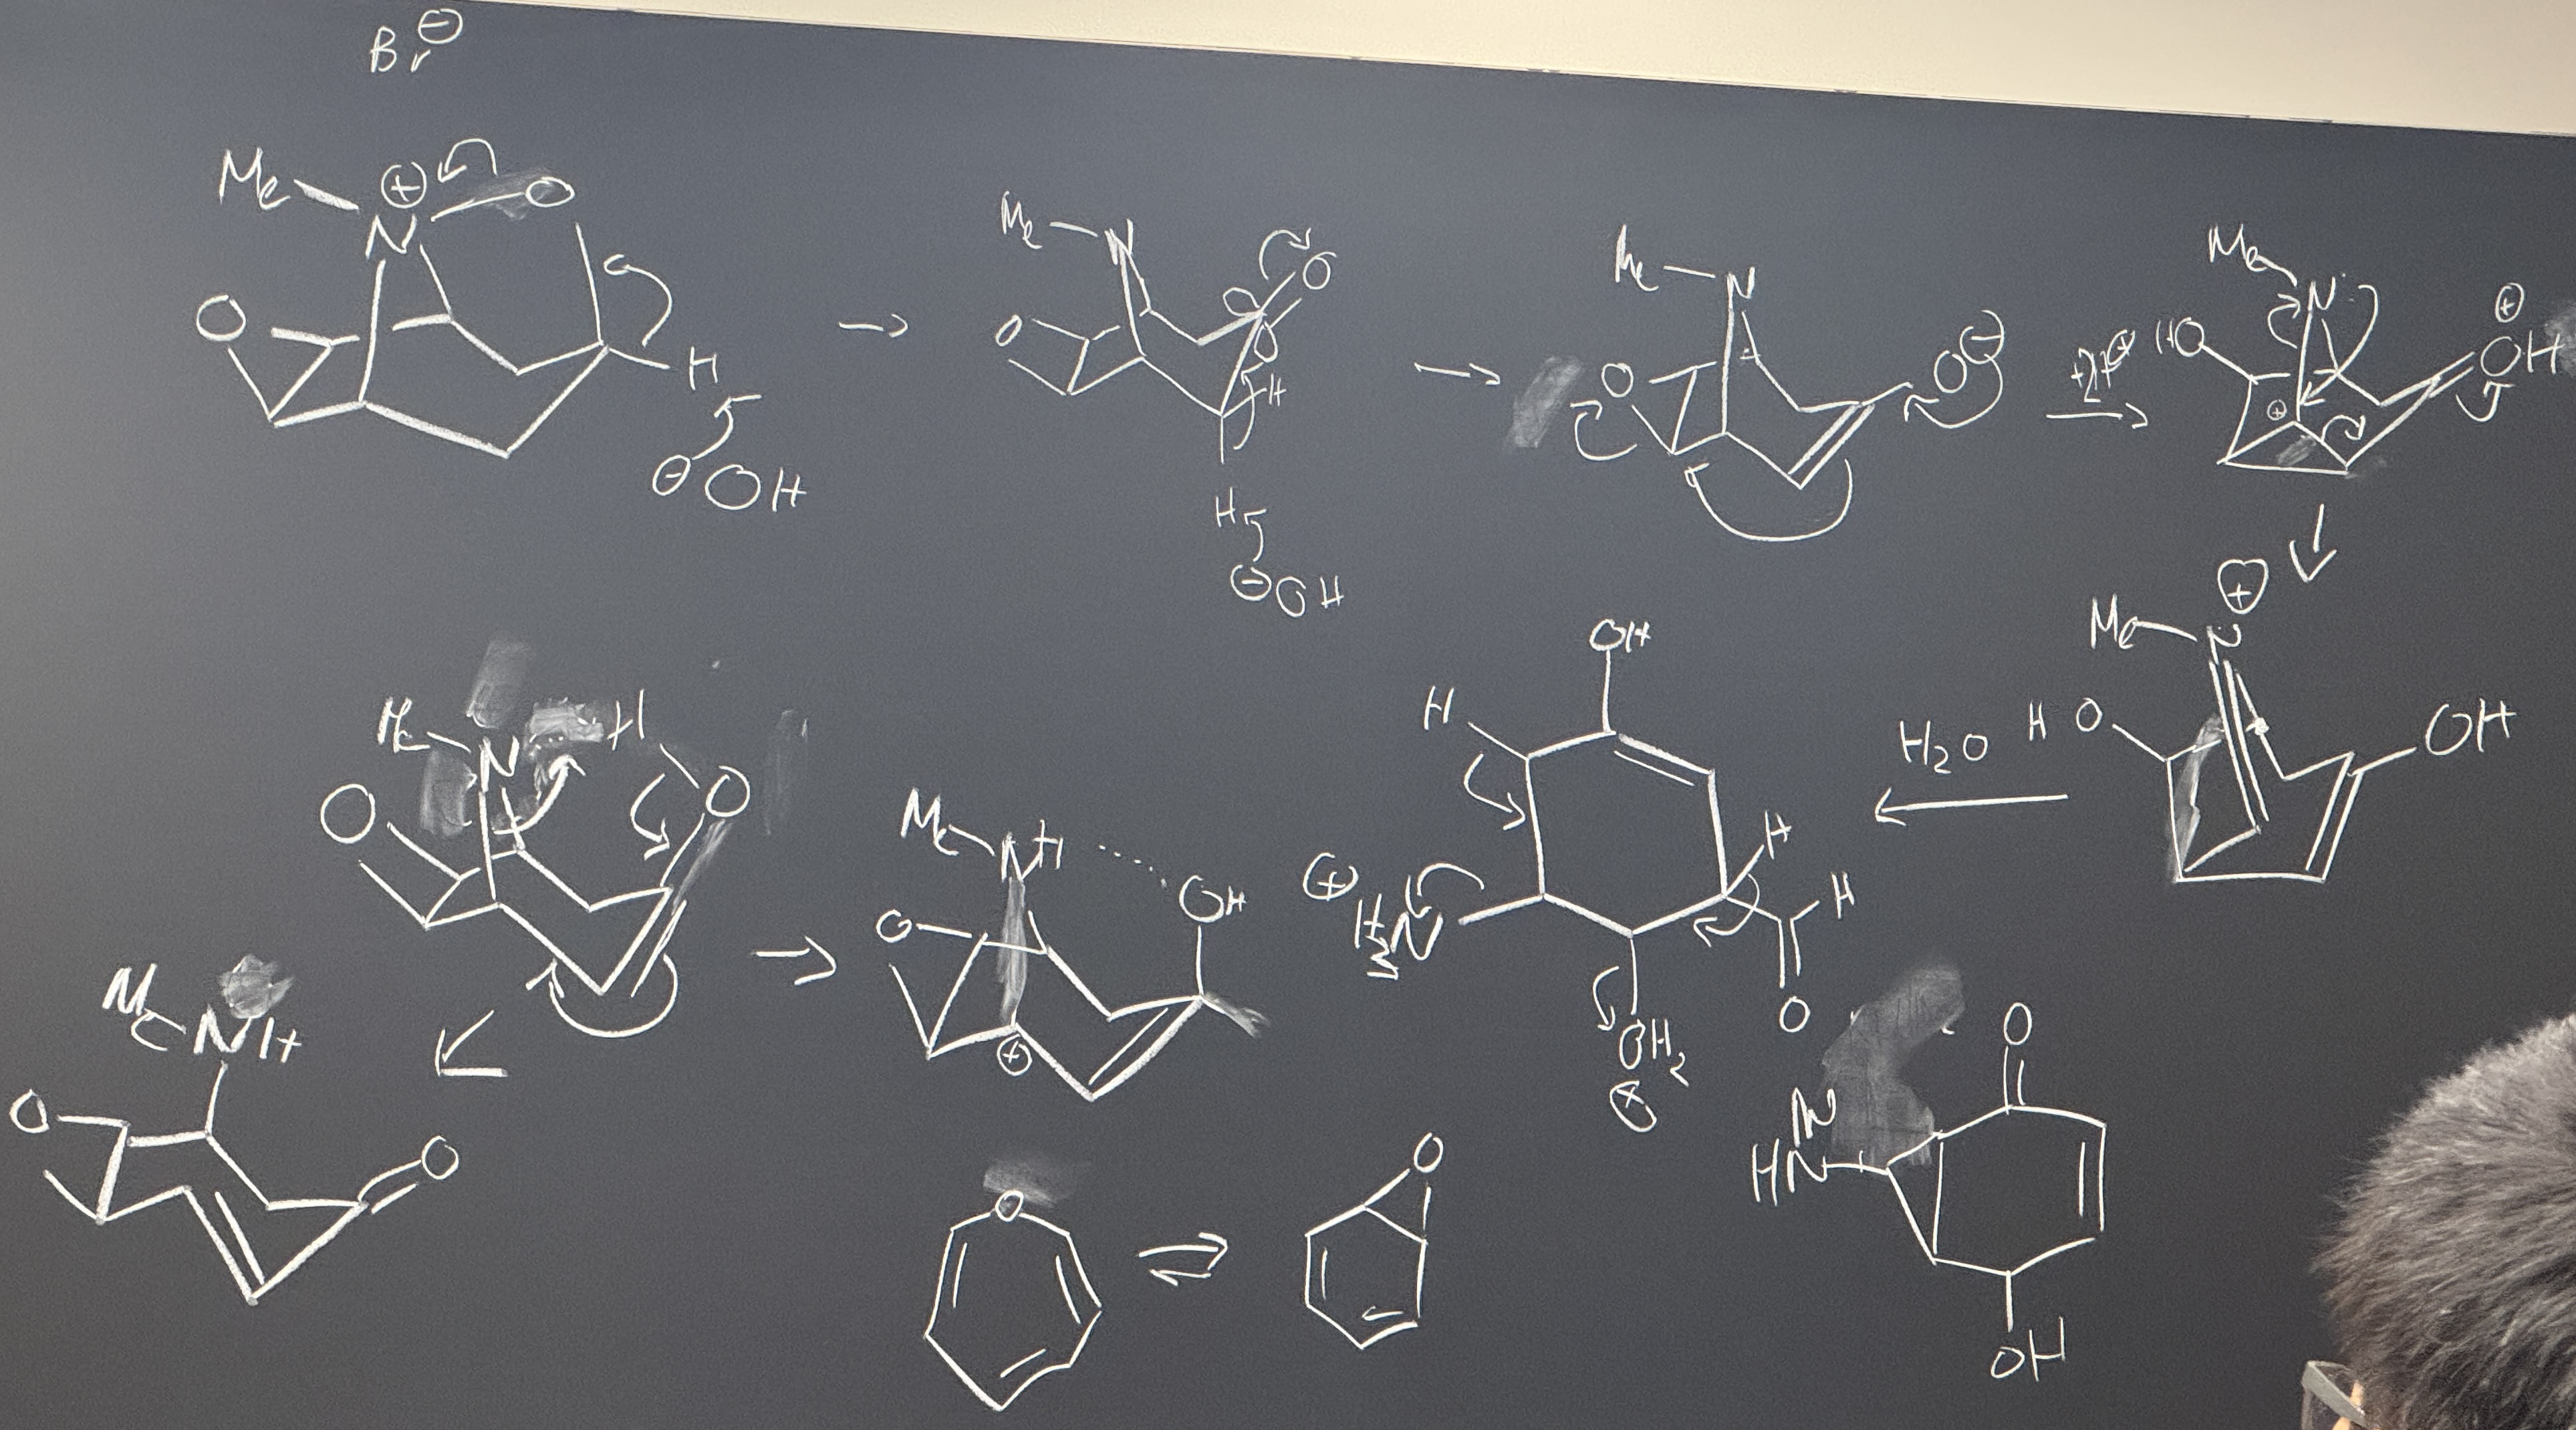
\includegraphics[width=0.8\linewidth]{WPSet1Q7S.JPG}
        \caption{Wendlandt PSet 1, Q7 solution.}
        \label{fig:WPSet1Q7S}
    \end{figure}
    \pagebreak
    \item We now begin discussing Problem 5.
    \begin{figure}[h!]
        \centering
        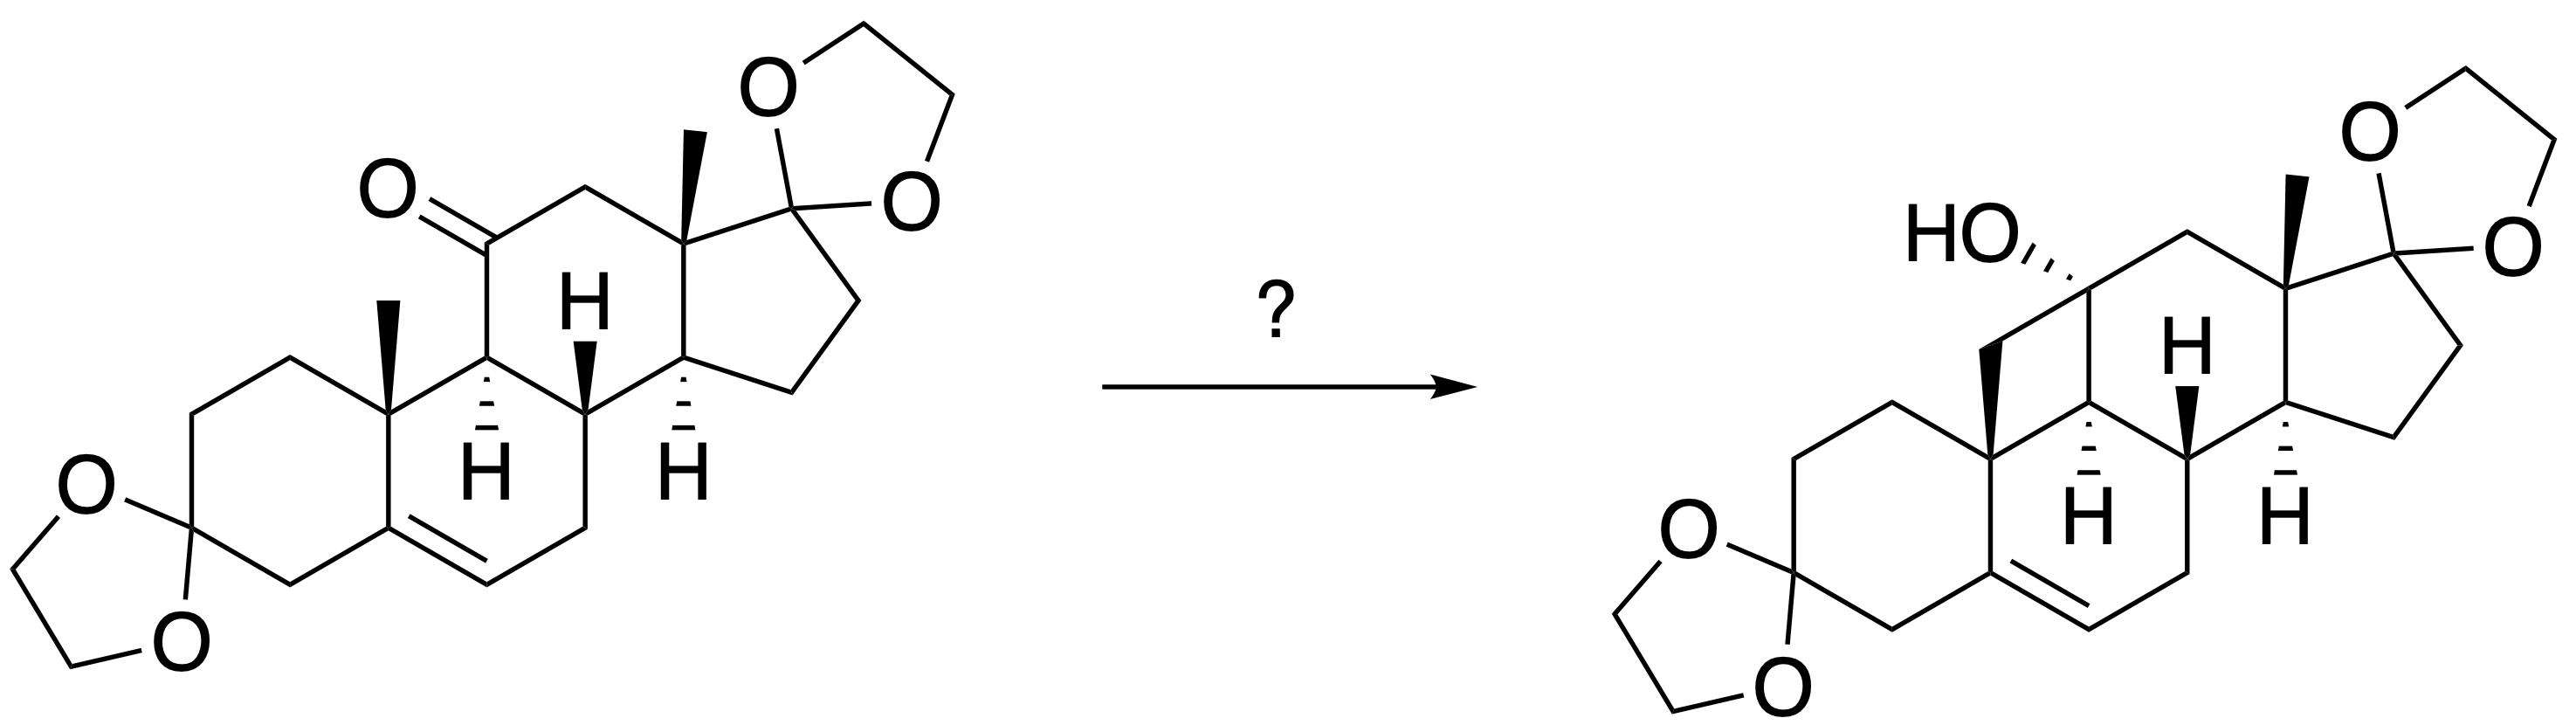
\includegraphics[width=0.55\linewidth]{WPSet1Q5.png}
        \caption{Wendlandt PSet 1, Q5.}
        \label{fig:WPSet1Q5}
    \end{figure}
    \item \textbf{Noorish 2 reaction}.
    \item Why is \ce{O*} less stable than \ce{C*}?
    \begin{itemize}
        \item Bond dissociation energies.
        \item \SI{10}{\kilo\calorie\per\mole} driving force to form \ce{O-H} and break \ce{C-H}.
        \item \SI{50}{\kilo\calorie\per\mole} favorability for deprotonating isopropanol at the alcohol vs. the methine \ce{C-H}.
        \begin{itemize}
            \item Derived by 35-fold difference in $\pKa$, so $\Delta G=-1.4\log(10^{35})\approx 50$.
        \end{itemize}
    \end{itemize}
    \item Altogether, the full solution to PSet 1, Q5 is on the next page.
    \begin{figure}[h!]
        \centering
        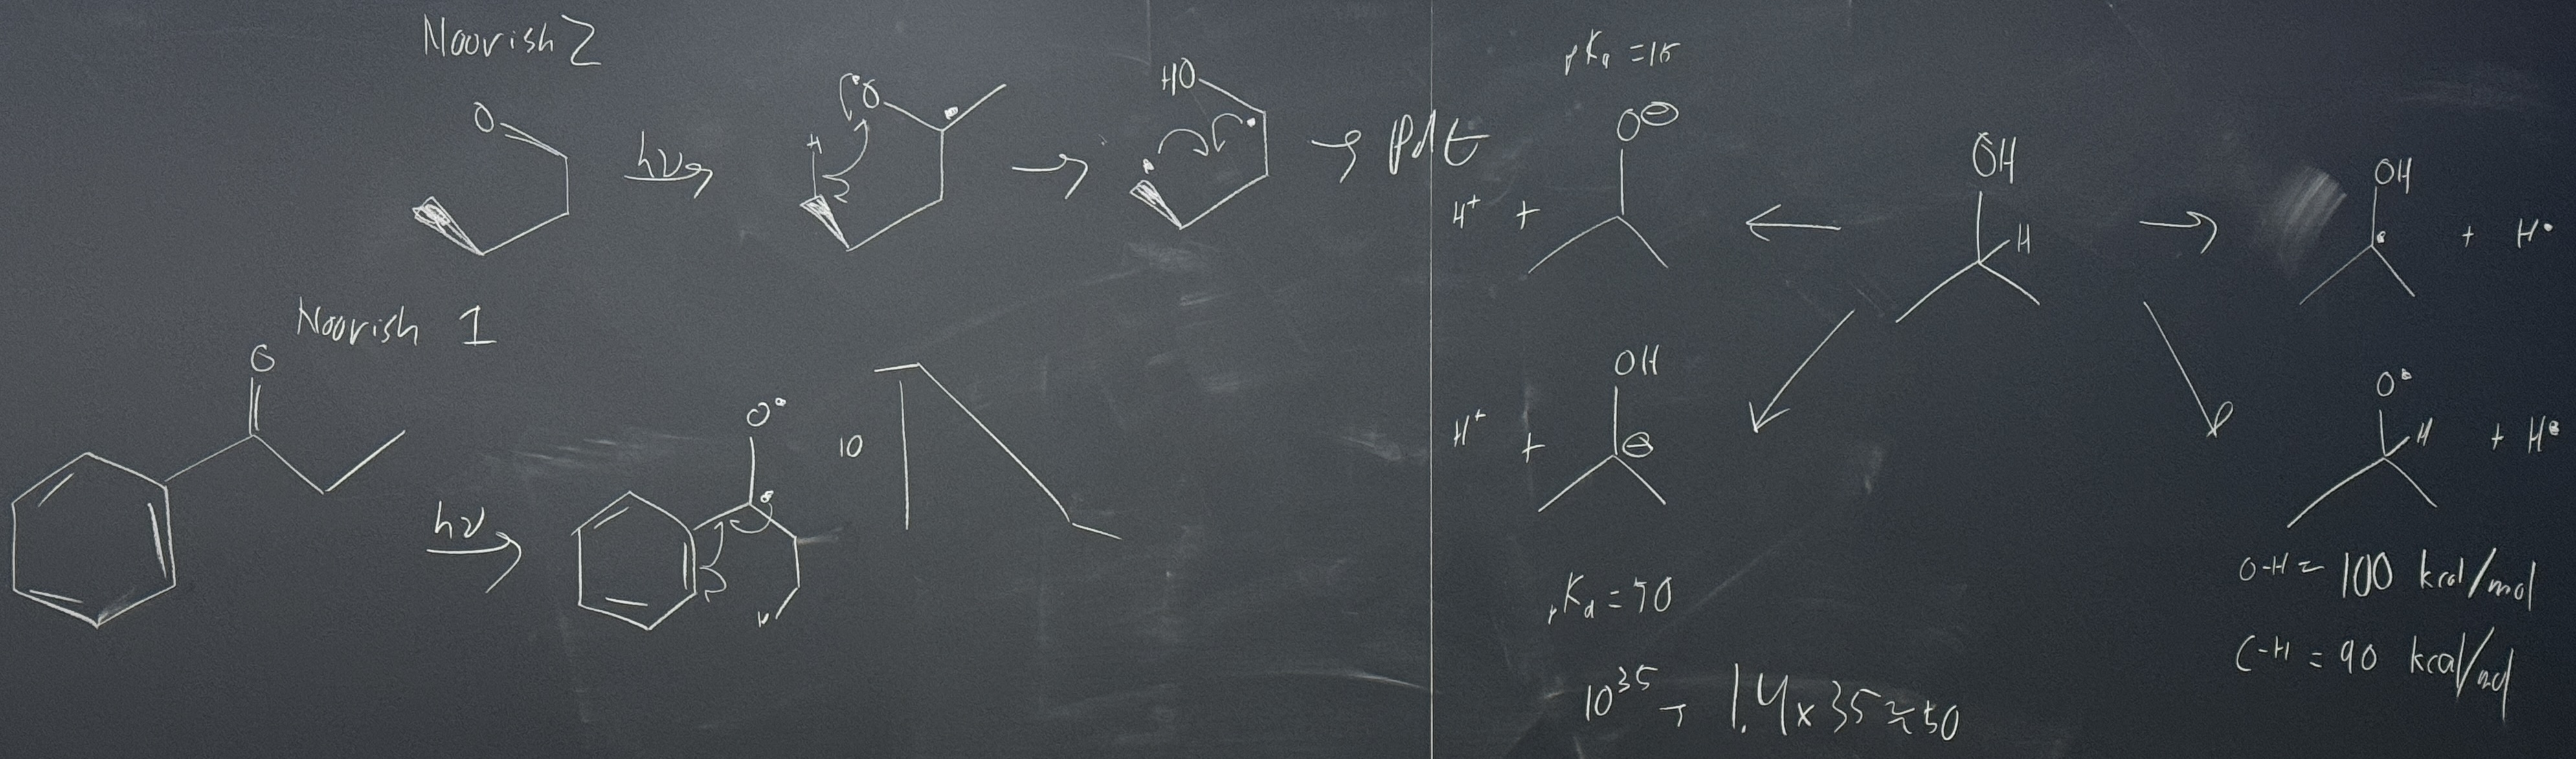
\includegraphics[width=0.8\linewidth]{WPSet1Q5S.JPG}
        \caption{Wendlandt PSet 1, Q5 solution.}
        \label{fig:WPSet1Q5S}
    \end{figure}
    \pagebreak
    \item We now begin discussing Problem 3.
    \begin{figure}[h!]
        \centering
        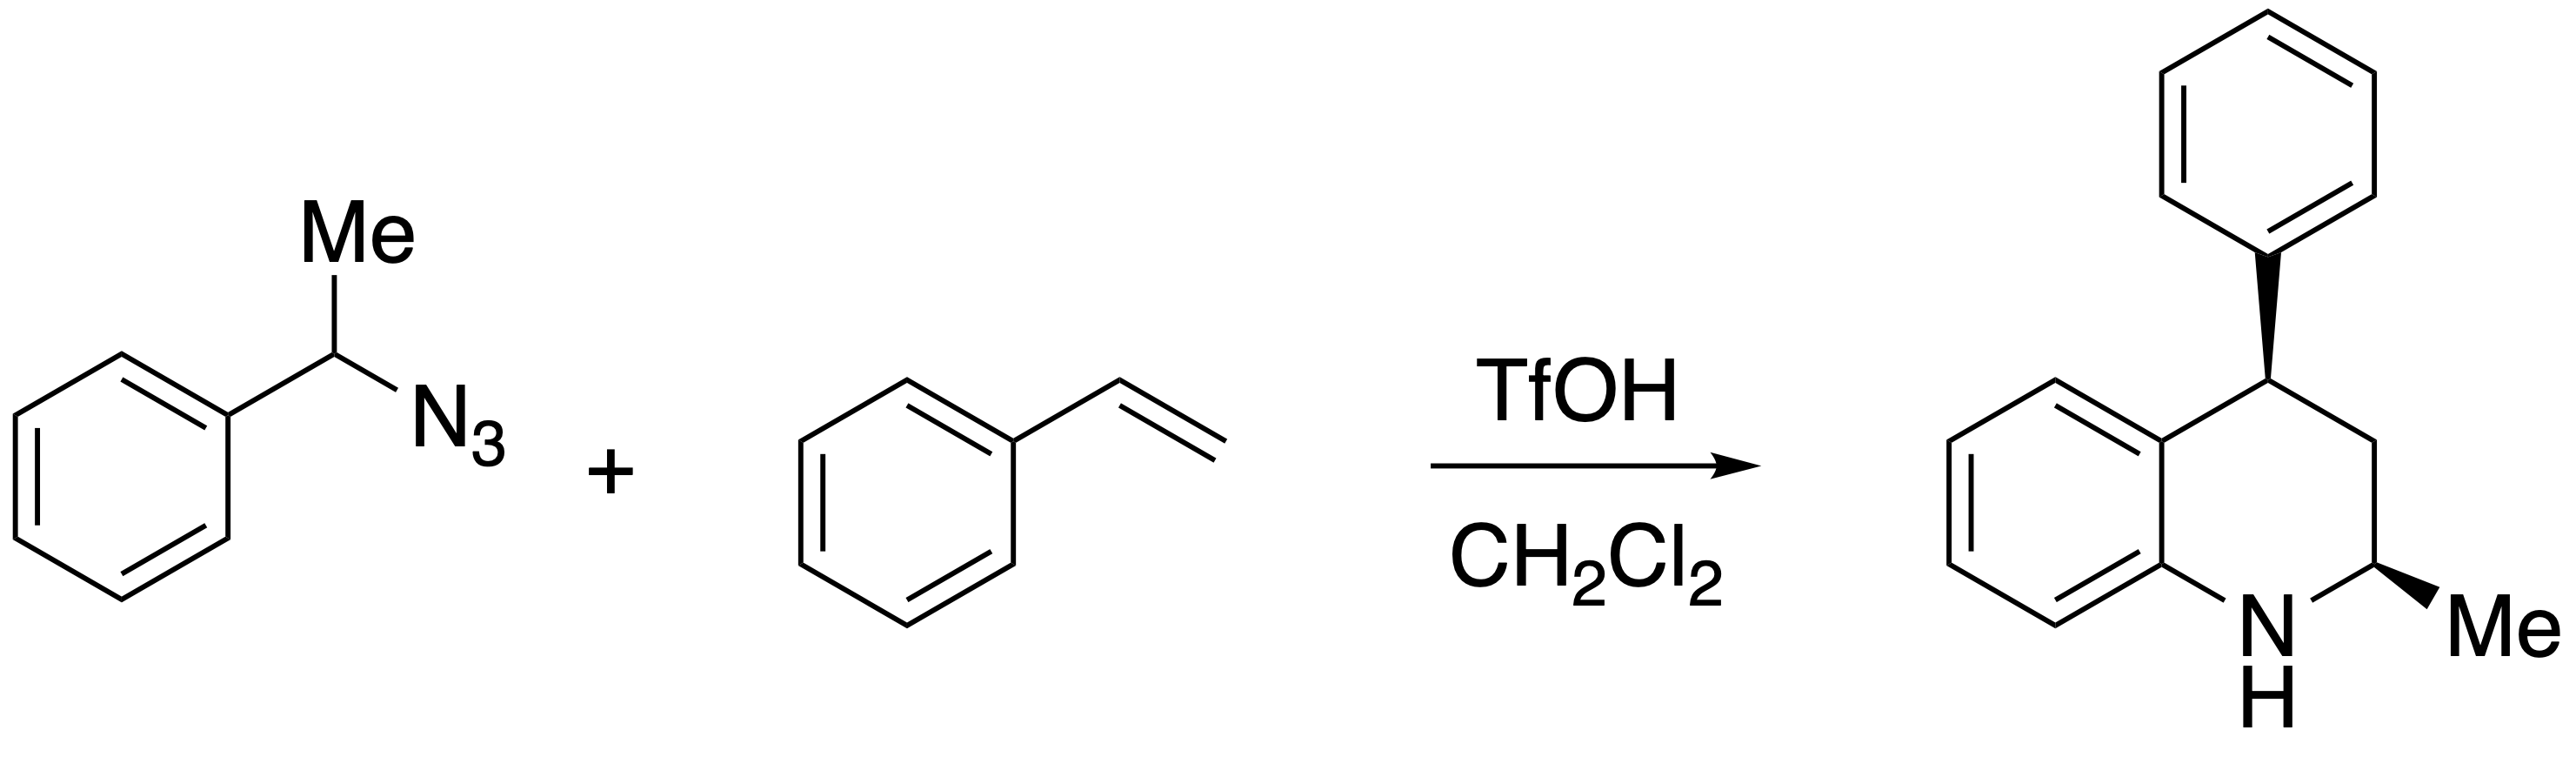
\includegraphics[width=0.55\linewidth]{WPSet1Q3.png}
        \caption{Wendlandt PSet 1, Q3.}
        \label{fig:WPSet1Q3}
    \end{figure}
    \item This reaction has a name, per Alison.
    \item When can \ce{C-C} bonds migrate?
    \item The second resonance structure explains why you protonate the internal nitrogen instead of the terminal one.
    \item The second step is $\alpha$-elimination; electrons flow from the atom to itself.
    \item Aside: Drawing an unprotonated \textbf{nitrene} (nitrogen analogue of a carbene).
    \begin{itemize}
        \item Nitrenes are electrophiles because they have one lone pair and two unpaired electrons.
        \item Nitrenes are $sp^2$-hybridized; we know this because ??.
        \begin{itemize}
            \item We'll cover this next time.
            \item 3 vs. 2 regions of electron density?
        \end{itemize}
        \item Lone pair in both $sp^2$ orbitals, vs. lone pair in one $sp$-orbital and two single electrons in orthogonal $p$ orbitals. Singlet vs. triplet nitrene.
        \item Triplet nitrene is low energy per Hund's rule; singlet nitrene is higher energy.
        \item Orbital mixing in singlet vs. triplet states. Draw an MO diagram! Next time, we'll build MOs from the ground up for nitrene.
    \end{itemize}
    \item Altogether, the full solution to PSet 1, Q3 is on the next page.
    \begin{figure}[h!]
        \centering
        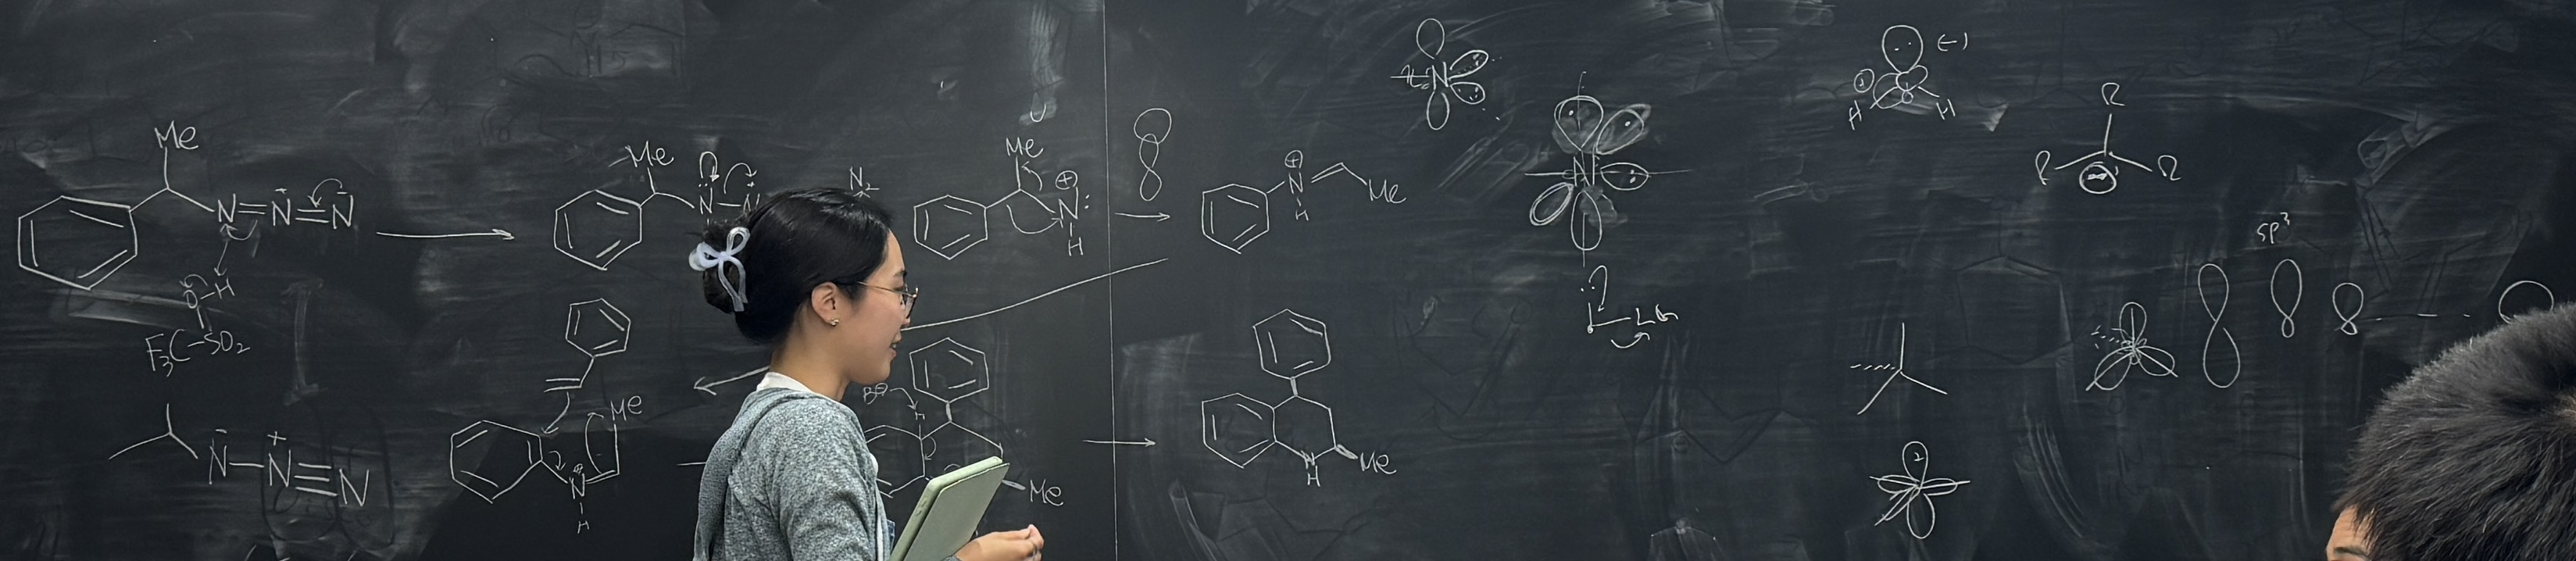
\includegraphics[width=0.8\linewidth]{WPSet1Q3S.JPG}
        \caption{Wendlandt PSet 1, Q3 solution.}
        \label{fig:WPSet1Q3S}
    \end{figure}
    \pagebreak
    \item Alison will send out PSet 2 over the weekend.
\end{itemize}




\end{document}